% Options for packages loaded elsewhere
\PassOptionsToPackage{unicode}{hyperref}
\PassOptionsToPackage{hyphens}{url}
%
\documentclass[
]{book}
\usepackage{amsmath,amssymb}
\usepackage{lmodern}
\usepackage{ifxetex,ifluatex}
\ifnum 0\ifxetex 1\fi\ifluatex 1\fi=0 % if pdftex
  \usepackage[T1]{fontenc}
  \usepackage[utf8]{inputenc}
  \usepackage{textcomp} % provide euro and other symbols
\else % if luatex or xetex
  \usepackage{unicode-math}
  \defaultfontfeatures{Scale=MatchLowercase}
  \defaultfontfeatures[\rmfamily]{Ligatures=TeX,Scale=1}
\fi
% Use upquote if available, for straight quotes in verbatim environments
\IfFileExists{upquote.sty}{\usepackage{upquote}}{}
\IfFileExists{microtype.sty}{% use microtype if available
  \usepackage[]{microtype}
  \UseMicrotypeSet[protrusion]{basicmath} % disable protrusion for tt fonts
}{}
\makeatletter
\@ifundefined{KOMAClassName}{% if non-KOMA class
  \IfFileExists{parskip.sty}{%
    \usepackage{parskip}
  }{% else
    \setlength{\parindent}{0pt}
    \setlength{\parskip}{6pt plus 2pt minus 1pt}}
}{% if KOMA class
  \KOMAoptions{parskip=half}}
\makeatother
\usepackage{xcolor}
\IfFileExists{xurl.sty}{\usepackage{xurl}}{} % add URL line breaks if available
\IfFileExists{bookmark.sty}{\usepackage{bookmark}}{\usepackage{hyperref}}
\hypersetup{
  pdftitle={A Minimal Book Example},
  pdfauthor={John Doe},
  hidelinks,
  pdfcreator={LaTeX via pandoc}}
\urlstyle{same} % disable monospaced font for URLs
\usepackage{color}
\usepackage{fancyvrb}
\newcommand{\VerbBar}{|}
\newcommand{\VERB}{\Verb[commandchars=\\\{\}]}
\DefineVerbatimEnvironment{Highlighting}{Verbatim}{commandchars=\\\{\}}
% Add ',fontsize=\small' for more characters per line
\usepackage{framed}
\definecolor{shadecolor}{RGB}{248,248,248}
\newenvironment{Shaded}{\begin{snugshade}}{\end{snugshade}}
\newcommand{\AlertTok}[1]{\textcolor[rgb]{0.94,0.16,0.16}{#1}}
\newcommand{\AnnotationTok}[1]{\textcolor[rgb]{0.56,0.35,0.01}{\textbf{\textit{#1}}}}
\newcommand{\AttributeTok}[1]{\textcolor[rgb]{0.77,0.63,0.00}{#1}}
\newcommand{\BaseNTok}[1]{\textcolor[rgb]{0.00,0.00,0.81}{#1}}
\newcommand{\BuiltInTok}[1]{#1}
\newcommand{\CharTok}[1]{\textcolor[rgb]{0.31,0.60,0.02}{#1}}
\newcommand{\CommentTok}[1]{\textcolor[rgb]{0.56,0.35,0.01}{\textit{#1}}}
\newcommand{\CommentVarTok}[1]{\textcolor[rgb]{0.56,0.35,0.01}{\textbf{\textit{#1}}}}
\newcommand{\ConstantTok}[1]{\textcolor[rgb]{0.00,0.00,0.00}{#1}}
\newcommand{\ControlFlowTok}[1]{\textcolor[rgb]{0.13,0.29,0.53}{\textbf{#1}}}
\newcommand{\DataTypeTok}[1]{\textcolor[rgb]{0.13,0.29,0.53}{#1}}
\newcommand{\DecValTok}[1]{\textcolor[rgb]{0.00,0.00,0.81}{#1}}
\newcommand{\DocumentationTok}[1]{\textcolor[rgb]{0.56,0.35,0.01}{\textbf{\textit{#1}}}}
\newcommand{\ErrorTok}[1]{\textcolor[rgb]{0.64,0.00,0.00}{\textbf{#1}}}
\newcommand{\ExtensionTok}[1]{#1}
\newcommand{\FloatTok}[1]{\textcolor[rgb]{0.00,0.00,0.81}{#1}}
\newcommand{\FunctionTok}[1]{\textcolor[rgb]{0.00,0.00,0.00}{#1}}
\newcommand{\ImportTok}[1]{#1}
\newcommand{\InformationTok}[1]{\textcolor[rgb]{0.56,0.35,0.01}{\textbf{\textit{#1}}}}
\newcommand{\KeywordTok}[1]{\textcolor[rgb]{0.13,0.29,0.53}{\textbf{#1}}}
\newcommand{\NormalTok}[1]{#1}
\newcommand{\OperatorTok}[1]{\textcolor[rgb]{0.81,0.36,0.00}{\textbf{#1}}}
\newcommand{\OtherTok}[1]{\textcolor[rgb]{0.56,0.35,0.01}{#1}}
\newcommand{\PreprocessorTok}[1]{\textcolor[rgb]{0.56,0.35,0.01}{\textit{#1}}}
\newcommand{\RegionMarkerTok}[1]{#1}
\newcommand{\SpecialCharTok}[1]{\textcolor[rgb]{0.00,0.00,0.00}{#1}}
\newcommand{\SpecialStringTok}[1]{\textcolor[rgb]{0.31,0.60,0.02}{#1}}
\newcommand{\StringTok}[1]{\textcolor[rgb]{0.31,0.60,0.02}{#1}}
\newcommand{\VariableTok}[1]{\textcolor[rgb]{0.00,0.00,0.00}{#1}}
\newcommand{\VerbatimStringTok}[1]{\textcolor[rgb]{0.31,0.60,0.02}{#1}}
\newcommand{\WarningTok}[1]{\textcolor[rgb]{0.56,0.35,0.01}{\textbf{\textit{#1}}}}
\usepackage{longtable,booktabs,array}
\usepackage{calc} % for calculating minipage widths
% Correct order of tables after \paragraph or \subparagraph
\usepackage{etoolbox}
\makeatletter
\patchcmd\longtable{\par}{\if@noskipsec\mbox{}\fi\par}{}{}
\makeatother
% Allow footnotes in longtable head/foot
\IfFileExists{footnotehyper.sty}{\usepackage{footnotehyper}}{\usepackage{footnote}}
\makesavenoteenv{longtable}
\usepackage{graphicx}
\makeatletter
\def\maxwidth{\ifdim\Gin@nat@width>\linewidth\linewidth\else\Gin@nat@width\fi}
\def\maxheight{\ifdim\Gin@nat@height>\textheight\textheight\else\Gin@nat@height\fi}
\makeatother
% Scale images if necessary, so that they will not overflow the page
% margins by default, and it is still possible to overwrite the defaults
% using explicit options in \includegraphics[width, height, ...]{}
\setkeys{Gin}{width=\maxwidth,height=\maxheight,keepaspectratio}
% Set default figure placement to htbp
\makeatletter
\def\fps@figure{htbp}
\makeatother
\setlength{\emergencystretch}{3em} % prevent overfull lines
\providecommand{\tightlist}{%
  \setlength{\itemsep}{0pt}\setlength{\parskip}{0pt}}
\setcounter{secnumdepth}{5}
\usepackage{booktabs}
\ifluatex
  \usepackage{selnolig}  % disable illegal ligatures
\fi
\usepackage[]{natbib}
\bibliographystyle{plainnat}

\title{A Minimal Book Example}
\author{John Doe}
\date{2022-05-07}

\begin{document}
\maketitle

{
\setcounter{tocdepth}{1}
\tableofcontents
}
\begin{Shaded}
\begin{Highlighting}[]
\NormalTok{bookdown}\SpecialCharTok{::}\FunctionTok{render\_book}\NormalTok{()}
\end{Highlighting}
\end{Shaded}

\begin{Shaded}
\begin{Highlighting}[]
\NormalTok{bookdown}\SpecialCharTok{::}\FunctionTok{serve\_book}\NormalTok{()}
\end{Highlighting}
\end{Shaded}

\hypertarget{introduction-to-kriging}{%
\chapter{Introduction to Kriging}\label{introduction-to-kriging}}

克里金法(Kriging)是一種用於空間資料的插值方法,通常視為高斯過程回歸或者 BLUP。

\hypertarget{assumption}{%
\section{Assumption}\label{assumption}}

固有平穩過程 (intrinsically stationary process)

\begin{itemize}
\tightlist
\item
  數學期望與地理位置無關,即觀察任一小區域他的屬性應當相同 (constant mean or variance)
\item
  半方差函數只與距離有關,即觀察任一小區域他的 Variogram 應當相同 (constant variogram)
\end{itemize}

若未滿足假設(可由 Voronoi 圖檢驗),可以對資料做轉換 (log transformation of squared)

\hypertarget{pros-and-cons}{%
\subsection*{Pros and cons}\label{pros-and-cons}}
\addcontentsline{toc}{subsection}{Pros and cons}

\begin{itemize}
\tightlist
\item
  Pros : kriging model 告訴我們感興趣的空間特徵均值,且是最佳無偏 (BLUP),並且可以估計誤差範圍
\item
  Cons : 每當你要重新估計其他區域的資料,你的線性系統要被完全更新
\end{itemize}

\hypertarget{relation-to-gpr}{%
\subsection*{Relation to GPR}\label{relation-to-gpr}}
\addcontentsline{toc}{subsection}{Relation to GPR}

\begin{itemize}
\tightlist
\item
  GPR : 隨機場為高斯過程
\item
  Kriging : 隨機場為固有平穩過程
\end{itemize}

若協方差函數相同,則普通克里金與簡單克里金法與GPR利用正態分配的最大似然估計輸出相同

\hypertarget{blue-best-linear-unbiased-estimator}{%
\section{BLUE (Best Linear Unbiased Estimator)}\label{blue-best-linear-unbiased-estimator}}

通常我們稱克里金法為最佳無偏線性預測(BLUP) :\\
* \textbf{Best :} 最小變方 (最小方差)
* \textbf{Linear :} 估計值為觀測值的線性組合
* \textbf{Unbiased :} 估計值的期望值等於真值

\hypertarget{ux666eux901aux514bux91ccux91d1-ok-oridnary-kriging}{%
\subsection{普通克里金 (OK Oridnary Kriging)}\label{ux666eux901aux514bux91ccux91d1-ok-oridnary-kriging}}

我們相信空間資料與地理位置具有相關性,對於未知的某個空間資訊\(Y_0\),我們透過觀測其附近 \(n\) 個位置 \(s_1,\cdots,s_n\) 的 \(n\) 個空間資訊 \(Y\) 來線性組合估計 \(Y_0\),及以下表述 :
\[
\hat Y(s_0) = \sum_{i=1}^n\lambda_iY(s_i) \tag 1
\]

現在我們只要找出權重係數 \(\lambda_i\) 就能解決問題了!,為了滿足無偏的性質,\textbf{普通克里金(Oridnary Kriging)} 假設空間資訊在每一個地理位置都有相同的相同期望值 (constant unknown mean),即\textbf{數學期望值與空間位置無關}

\[
Y(\mathbf{s}) = \mu + \delta(\mathbf{s})\tag 2
\]

其中 \(E(Y) = \mu\) 且 \(\delta\) (平均為0的固有平穩過程) 為地理位置 \(\mathbf{s}\),\(Y\) 與 \(\hat Y\) 的誤差

\[
E(\hat Y(s_0)) = \mu = \mu\sum\lambda_i \iff \sum \lambda_i = 1 \tag 3
\]

為了滿足在限制條件 \((3)\) 下最佳化

\[
\arg\min_\lambda E(||\hat Y(s_0) - Y(s_0)||^2) \iff \arg\min_\lambda \frac{1}{2}E(||\sum_{i=1}^n\lambda_iY(s_i) -Y(s_0)||^2) \\
\mbox{subject to } \sum_{i=1}^n\lambda_i = 1 \tag 4
\]

利用拉格朗日乘數 \(L(\lambda_1,\cdots,\lambda_n,\phi)\) 可得,詳見 \href{http://www1.mate.polimi.it/~bonavent/Homepage_Luca_file/lezkrig005.pdf}{克里金法原理與推導}

\[
\begin{bmatrix}
r_{11}&r_{12}&\cdots&r_{1n}&1\\ r_{21}&r_{22}&\cdots&r_{2n}&1\\
\cdots&\cdots&\cdots&\cdots&\cdots\\
r_{n1}&r_{n2}&\cdots&r_{nn}&1\\1&1&\cdots&1&0\end{bmatrix}
\begin{bmatrix} \lambda_1\\ \lambda_2\\\cdots\\\lambda_n\\-\phi\end{bmatrix}=\begin{bmatrix} r_{1o}\\ r_{2o}\\\cdots\\r_{no}\\1\end{bmatrix} \tag 5
\]

其中 \(r_{ij}\) 為半方差函數,\(\phi\) 為拉格朗日的限制參數,做完逆矩陣即可得權重係數

\[
\begin{bmatrix} \lambda_1\\ \lambda_2\\\cdots\\\lambda_n\\-\phi\end{bmatrix}=
\begin{bmatrix}
r_{11}&r_{12}&\cdots&r_{1n}&1\\ r_{21}&r_{22}&\cdots&r_{2n}&1\\
\cdots&\cdots&\cdots&\cdots&\cdots\\
r_{n1}&r_{n2}&\cdots&r_{nn}&1\\1&1&\cdots&1&0\end{bmatrix}^{-1}
\begin{bmatrix} r_{1o}\\ r_{2o}\\\cdots\\r_{no}\\1\end{bmatrix} \tag 6
\]

我們計做 \(\lambda_O = \Gamma_O^{-1}\gamma_O\),帶回原式我們可以估得誤差的方差為 \(\sigma^2_O =\lambda_O^\top\gamma_O= \gamma_O^\top \Gamma_O^{-1}\gamma_O\)

\hypertarget{ux534aux65b9ux5deeux5716-variogram}{%
\subsection{半方差圖 (Variogram)}\label{ux534aux65b9ux5deeux5716-variogram}}

半方差的定義為 \(r_{ij} = \frac{1}{2}E[(Y(s_i) - Y(s_j))^2]\),根據我們的假設,我們希望地理位置鄰近的地方具有相似的空間資訊,即 \(\mbox{Distance}\rightarrow 0 \implies r_{ij} \rightarrow 0\)

\textless img src=``\url{https://i.imgur.com/PWIf1LT.png}'',width=``600'',height=``400''\textgreater{}

半方差圖其中幾個重要的術語

\begin{itemize}
\tightlist
\item
  \textbf{Data :} 即 \(\frac{1}{2}(Y(s_i) - Y(s_j))^2\),為上圖中紅色標記點
\item
  \textbf{Variogram model :} 即是 Data 的擬合曲線,常用``線性''、``高斯''、``球面''、``指數''等逼近
\item
  \textbf{Nugget :} 用 \(C_o\) 表示,為距離最近兩點的半方差值

  \begin{itemize}
  \tightlist
  \item
    越大的 \(C_o\) 表示空間測量誤差越大
  \end{itemize}
\item
  \textbf{Sill :} 用 \(C_o + C\) 表示,當半方差函數達到一個穩定態時,該半方差值稱為 Sill
\item
  \textbf{Range :} 用 \(A_o\) 表示,達到 Sill 的距離,表示空間相關性的作用範圍

  \begin{itemize}
  \tightlist
  \item
    超過 \(A_o\) 我們稱空間相關性不存在,即不能使用內插法
  \end{itemize}
\end{itemize}

\hypertarget{ux7c21ux55aeux514bux91ccux91d1-sk-simple-kriging}{%
\subsection{簡單克里金 (SK Simple Kriging)}\label{ux7c21ux55aeux514bux91ccux91d1-sk-simple-kriging}}

不同於普通克里金法,簡單克里金假設未知點的偏差是由已知點的偏差線性組合(with known mean)
\[
\hat Y(s_0) - \mu = \sum_{i=1}^n\lambda_i(Y(s_i) - \mu)
\]
神奇的是,這個條件會自動滿足無偏性
\[
E(\hat Y_0) = E(\mu + \sum_{i=1}^n\lambda_i(Y(s_i) - \mu)) = \mu
\]
所以它不需要普通克里金法的限制 \((3)\)

\hypertarget{ux6cdbux514bux91ccux91d1-uk-universal-kriging}{%
\subsection{泛克里金 (UK Universal kriging)}\label{ux6cdbux514bux91ccux91d1-uk-universal-kriging}}

泛克里金法假設隨機場 \(Y\) 是由隨機場的漂移與固有平穩過程生成出來的

\[
Y(\mathbf{s}) = \sum_{i=1}^p\beta_if_i(\mathbf{s}) + \delta(\mathbf{s})
\]

注意到如果取 \(f_i = 1,p=1\) 則與普通克里金一樣,為了簡便說明,給出以下符號

\[
\mathbf{X} = \begin{bmatrix}f_1(s_1)&\cdots&f_p(s_1)\\f_1(s_2)&\cdots&f_p(s_2)\\\vdots&\cdots&\vdots\\f_1(s_n)&\cdots&f_p(s_n)\end{bmatrix},\mathbf{\beta} = \begin{bmatrix}\beta_1\\\vdots\\\beta_p\end{bmatrix} \\
\mathbf{\delta(s)} = \begin{bmatrix}\delta(s_1)\\\vdots\\\delta(s_n)\end{bmatrix}, \mathbf{Y} = \begin{bmatrix}Y(s_1)\\\vdots\\Y(s_n)\end{bmatrix}
\]

則有 \(\bf Y = X\beta + \delta\),同樣地,為了滿足無偏性,我們有以下限制條件
\[
E(Y) = \sum_{i=1}^p\beta_if_i(\mathbf{s}) \\
E(\hat Y(s_0)) = E(\sum_{i=1}^n\lambda_iY(s_i)) = \sum_{i=1}^n\lambda_i\sum_{j=1}^p\beta_jf_j(s_i) = \sum_{i=1}^p\beta_if_i(\mathbf{s_0}) \\
f_j(\mathbf{s}) = \sum_{i=1}^n\lambda_if_j(s_i) \mbox{ for } j = 1,\cdots,p \\
\sum_{i=1}^n\lambda_i = 1
\]
再根據拉格朗日乘數求解方程,詳見 \href{http://www1.mate.polimi.it/~bonavent/Homepage_Luca_file/lezkrig005.pdf}{克里金法原理與推導}
\[
L(\lambda_1,\cdots,\lambda_n,m_1,\cdots,m_p) = E[||\hat Y(s_0) - Y(s_0)||^2] - 2m_0(\sum_{i=1}^n\lambda_i-1) - 2\sum_{j=1}^pm_j(\sum_{i=1}^n\lambda_if_j(s_i) - f_j(s_0))
\]
即有
\[
\begin{bmatrix}
\lambda_1 \\
\vdots \\
\lambda_n \\
m_0 \\
m_1 \\
\vdots  \\
m_p
\end{bmatrix} = \begin{bmatrix}
r_{11}  & \cdots & r_{1n} &1& f_1(s_1) & \cdots & f_1(x_n)\\
 \vdots & \ddots & \vdots  &\vdots& \vdots & \cdots & \vdots\\
r_{n1}  & \cdots & r_{nn} &1& f_p(s_1) & \cdots & f_p(s_n)\\
1&\cdots&1&0&0&\cdots&0 \\
f_1(s_1)  & \cdots & f_1(s_n) &0& 0 & \cdots & 0\\
 \vdots & \ddots & \vdots &\vdots& \vdots & \ddots & \vdots\\
 f_p(s_1) & \cdots & f_p(s_n) & 0 & 0 & \cdots &0
\end{bmatrix}^{-1}\begin{bmatrix}
r_{10} \\
\vdots \\
r_{n0} \\
1 \\
f_1(s_0) \\
\vdots \\
f_p(s_0)
\end{bmatrix}
\]
我們計做 \(\lambda_U = \Gamma_U^{-1}\gamma_U\),帶回原式我們可以估得誤差的方差為 \(\sigma^2_U =\lambda_U^\top\gamma_U= \gamma_U^\top \Gamma_U^{-1}\gamma_U\)

更進一步,如果 \(Y\) 的協方差矩陣 \(\Sigma\) 已知,則根據廣義最小平方法,將空間資訊 \(Y\) 投影到主成分空間使得誤差的斜方差矩陣沒有外部協方差,則有
\[
\hat\beta_{gls} = (X^\top\Sigma^{-1} X)^{-1}X^\top\Sigma^{-1} Y
\]

\hypertarget{ux5354ux540cux514bux91ccux91d1-ck-co-kriging}{%
\subsection{協同克里金 (CK Co-Kriging)}\label{ux5354ux540cux514bux91ccux91d1-ck-co-kriging}}

協同克里金是克里金法在多變量分析的衍生,協同克里金允許多個空間資訊 \(Y_1,\cdots,Y_K\) 分別在地理位置 \(\{s_1,\cdots,s_{n_k}\}, k=1,\cdots,K\) 被觀測到,則

\[
\hat Y(s_0) = \sum_{k=1}^K\sum_{i=1}^{n_k}\lambda_{k_i}Y_k(s_i)
\]

\hypertarget{ux6790ux53d6ux514bux91ccux91d1-dk-disjunctive-kriging}{%
\subsection{析取克里金 (DK Disjunctive Kriging)}\label{ux6790ux53d6ux514bux91ccux91d1-dk-disjunctive-kriging}}

析取克里金是隨機場的非線性估計,注意,在此之前都是線性估計!!

\[
\hat Y(s_0) = \sum_{i=1}^nf_i(Y(s_i))
\]

如果 \(f_i\) 為指示函數,則析取克里金又稱為指示克里金 (IK Indicator Kriging)

\hypertarget{r-ux8a9eux8a00ux5be6ux4f5c}{%
\section{R 語言實作}\label{r-ux8a9eux8a00ux5be6ux4f5c}}

\begin{enumerate}
\def\labelenumi{\arabic{enumi}.}
\tightlist
\item
  選定資料集與載入套件
\end{enumerate}

\begin{Shaded}
\begin{Highlighting}[]
\FunctionTok{library}\NormalTok{(gstat) }\CommentTok{\# for kriging}
\FunctionTok{library}\NormalTok{(sp) }\CommentTok{\# for meuse dataset}
\FunctionTok{library}\NormalTok{(FRK) }\CommentTok{\# for gird and fixed rank kriging }
\FunctionTok{library}\NormalTok{(tidyverse) }\CommentTok{\# for data flow}
\FunctionTok{library}\NormalTok{(gridExtra) }\CommentTok{\# for combine plot}
\FunctionTok{data}\NormalTok{(meuse)}
\end{Highlighting}
\end{Shaded}

\begin{enumerate}
\def\labelenumi{\arabic{enumi}.}
\setcounter{enumi}{1}
\tightlist
\item
  將資料轉成 SP 格式
\end{enumerate}

\begin{Shaded}
\begin{Highlighting}[]
\FunctionTok{coordinates}\NormalTok{(meuse) }\OtherTok{=} \ErrorTok{\textasciitilde{}}\NormalTok{ x }\SpecialCharTok{+}\NormalTok{ y}
\end{Highlighting}
\end{Shaded}

\begin{enumerate}
\def\labelenumi{\arabic{enumi}.}
\setcounter{enumi}{2}
\tightlist
\item
  建立要預測地點的網格
\end{enumerate}

\begin{Shaded}
\begin{Highlighting}[]
\NormalTok{GridBAUs }\OtherTok{\textless{}{-}} \FunctionTok{auto\_BAUs}\NormalTok{(}\AttributeTok{manifold =} \FunctionTok{plane}\NormalTok{(), }\CommentTok{\# 2D plane}
                       \AttributeTok{cellsize =} \FunctionTok{c}\NormalTok{(}\DecValTok{100}\NormalTok{,}\DecValTok{100}\NormalTok{), }\CommentTok{\# BAU cellsize}
                       \AttributeTok{type =} \StringTok{"grid"}\NormalTok{, }\CommentTok{\# grid (not hex)}
                       \AttributeTok{data =}\NormalTok{ meuse, }\CommentTok{\# data around which to create BAUs}
                       \AttributeTok{convex=}\SpecialCharTok{{-}}\FloatTok{0.05}\NormalTok{, }\CommentTok{\# border buffer factor}
                       \AttributeTok{nonconvex\_hull=}\ConstantTok{FALSE}\NormalTok{) }\CommentTok{\# convex hull}
\end{Highlighting}
\end{Shaded}

\hypertarget{ux53cdux8dddux96e2ux6b0aux91cdux63d2ux503cux6cd5}{%
\subsubsection{反距離權重插值法}\label{ux53cdux8dddux96e2ux6b0aux91cdux63d2ux503cux6cd5}}

\begin{Shaded}
\begin{Highlighting}[]
\NormalTok{idw2 }\OtherTok{\textless{}{-}} \FunctionTok{idw}\NormalTok{(}\AttributeTok{formula =} \FunctionTok{log}\NormalTok{(zinc) }\SpecialCharTok{\textasciitilde{}} \DecValTok{1}\NormalTok{, }\CommentTok{\# formula}
         \AttributeTok{locations =}\NormalTok{ meuse, }\CommentTok{\# data with measurements}
         \AttributeTok{newdata =}\NormalTok{ GridBAUs, }\CommentTok{\# where to be interpolated}
         \AttributeTok{nmin =} \DecValTok{0}\NormalTok{, }\CommentTok{\# the least numbers of data to be interpolated,}
         \AttributeTok{nmax =} \ConstantTok{Inf}\NormalTok{, }\CommentTok{\# the largest numbers of data to be interpolated,}
         \AttributeTok{maxdist =} \ConstantTok{Inf}\NormalTok{, }\CommentTok{\# the maximum distance of datat to be interpolated}
         \AttributeTok{idp =} \DecValTok{2}\NormalTok{, }\CommentTok{\# the distance attenuation parameter}
\NormalTok{         ) }
\end{Highlighting}
\end{Shaded}

\begin{verbatim}
## [inverse distance weighted interpolation]
\end{verbatim}

\begin{enumerate}
\def\labelenumi{\arabic{enumi}.}
\setcounter{enumi}{3}
\tightlist
\item
  建立半方差模型
\end{enumerate}

\begin{Shaded}
\begin{Highlighting}[]
\NormalTok{lzn.vgm }\OtherTok{\textless{}{-}} \FunctionTok{variogram}\NormalTok{(}\FunctionTok{log}\NormalTok{(zinc)}\SpecialCharTok{\textasciitilde{}}\DecValTok{1}\NormalTok{, meuse) }\CommentTok{\# calculates sample variogram values}
\NormalTok{lzn.model }\OtherTok{\textless{}{-}} \FunctionTok{vgm}\NormalTok{(}\AttributeTok{psill =} \DecValTok{1}\NormalTok{, }\CommentTok{\# create model}
                 \AttributeTok{model =} \StringTok{"Sph"}\NormalTok{, }\CommentTok{\# "Sph", "Exp", "Gau", "Mat", "Pow"}
                 \AttributeTok{range =} \DecValTok{900}\NormalTok{, }
                 \AttributeTok{nugget =} \DecValTok{1}\NormalTok{)}
\NormalTok{lzn.fit }\OtherTok{\textless{}{-}} \FunctionTok{fit.variogram}\NormalTok{(lzn.vgm, lzn.model) }\CommentTok{\# fit model}
\FunctionTok{plot}\NormalTok{(lzn.vgm, lzn.fit)}
\end{Highlighting}
\end{Shaded}

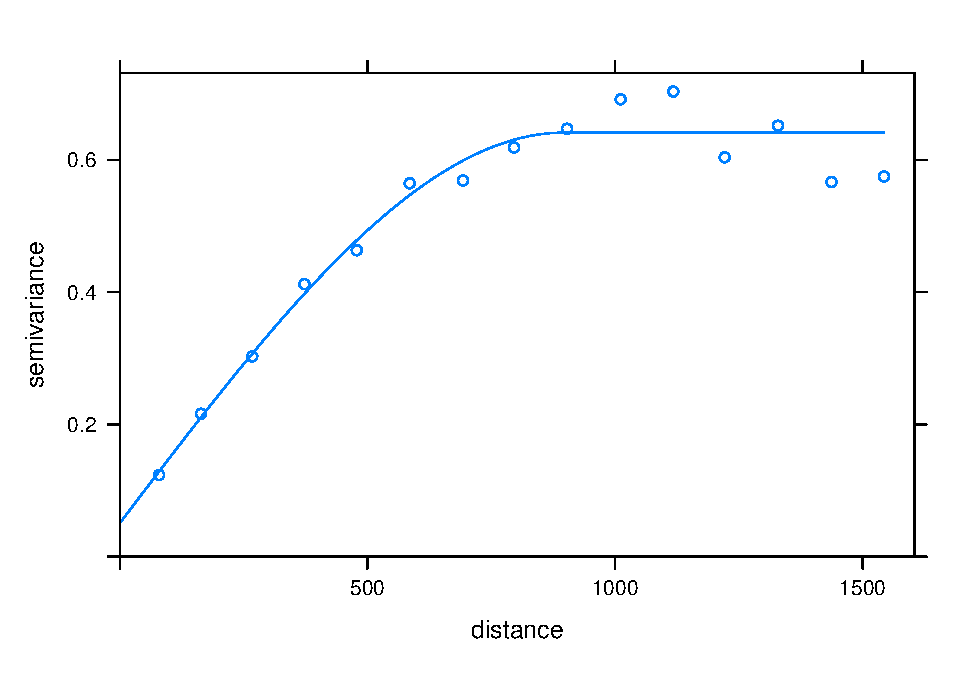
\includegraphics{_main_files/figure-latex/unnamed-chunk-8-1.pdf}

\hypertarget{ux5efaux7acbux5404ux7a2eux514bux91ccux91d1ux6a21ux578b}{%
\subsubsection{建立各種克里金模型}\label{ux5efaux7acbux5404ux7a2eux514bux91ccux91d1ux6a21ux578b}}

\begin{Shaded}
\begin{Highlighting}[]
\NormalTok{OK }\OtherTok{\textless{}{-}} \FunctionTok{krige}\NormalTok{(}\FunctionTok{log}\NormalTok{(zinc) }\SpecialCharTok{\textasciitilde{}} \DecValTok{1}\NormalTok{, meuse, GridBAUs, }\AttributeTok{model=}\NormalTok{lzn.fit) }\CommentTok{\# Ordinary kriging}
\end{Highlighting}
\end{Shaded}

\begin{verbatim}
## [using ordinary kriging]
\end{verbatim}

\begin{Shaded}
\begin{Highlighting}[]
\NormalTok{UK }\OtherTok{\textless{}{-}} \FunctionTok{krige}\NormalTok{(}\FunctionTok{log}\NormalTok{(zinc) }\SpecialCharTok{\textasciitilde{}}\NormalTok{ x}\SpecialCharTok{+}\NormalTok{y, meuse, GridBAUs, }\AttributeTok{model =}\NormalTok{ lzn.fit) }\CommentTok{\# Universal kriging}
\end{Highlighting}
\end{Shaded}

\begin{verbatim}
## [using universal kriging]
\end{verbatim}

\begin{Shaded}
\begin{Highlighting}[]
\FunctionTok{lm}\NormalTok{(var1.pred }\SpecialCharTok{\textasciitilde{}}\NormalTok{ x }\SpecialCharTok{+}\NormalTok{ y, UK) }\CommentTok{\# Use Universal kriging to calaulate the coefficient}
\end{Highlighting}
\end{Shaded}

\begin{verbatim}
## 
## Call:
## lm(formula = var1.pred ~ x + y, data = UK)
## 
## Coefficients:
## (Intercept)            x            y  
##  -8.0324313   -0.0008891    0.0005250
\end{verbatim}

\begin{Shaded}
\begin{Highlighting}[]
\NormalTok{SK }\OtherTok{\textless{}{-}} \FunctionTok{krige}\NormalTok{(}\FunctionTok{log}\NormalTok{(zinc)}\SpecialCharTok{\textasciitilde{}}\NormalTok{x}\SpecialCharTok{+}\NormalTok{y, meuse, GridBAUs, lzn.fit, }
            \AttributeTok{beta =} \FunctionTok{c}\NormalTok{(}\SpecialCharTok{{-}}\FloatTok{8.0324313}\NormalTok{, }\SpecialCharTok{{-}}\FloatTok{0.0008891}\NormalTok{, }\FloatTok{0.0005250}\NormalTok{)) }\CommentTok{\# Simple kriging}
\end{Highlighting}
\end{Shaded}

\begin{verbatim}
## [using simple kriging]
\end{verbatim}

\begin{Shaded}
\begin{Highlighting}[]
\NormalTok{CK }\OtherTok{\textless{}{-}} \FunctionTok{gstat}\NormalTok{(}\ConstantTok{NULL}\NormalTok{, }\StringTok{"logCd"}\NormalTok{, }\FunctionTok{log}\NormalTok{(cadmium) }\SpecialCharTok{\textasciitilde{}} \DecValTok{1}\NormalTok{, meuse)}
\NormalTok{CK }\OtherTok{\textless{}{-}} \FunctionTok{gstat}\NormalTok{(CK, }\StringTok{"logCu"}\NormalTok{, }\FunctionTok{log}\NormalTok{(copper) }\SpecialCharTok{\textasciitilde{}} \DecValTok{1}\NormalTok{, meuse)}
\NormalTok{CK }\OtherTok{\textless{}{-}} \FunctionTok{gstat}\NormalTok{(CK, }\StringTok{"logPb"}\NormalTok{, }\FunctionTok{log}\NormalTok{(lead) }\SpecialCharTok{\textasciitilde{}} \DecValTok{1}\NormalTok{,meuse)}
\NormalTok{CK }\OtherTok{\textless{}{-}} \FunctionTok{gstat}\NormalTok{(CK, }\StringTok{"logZn"}\NormalTok{, }\FunctionTok{log}\NormalTok{(zinc) }\SpecialCharTok{\textasciitilde{}} \DecValTok{1}\NormalTok{,meuse)}
\NormalTok{CK.vgm }\OtherTok{\textless{}{-}} \FunctionTok{variogram}\NormalTok{(CK)}
\NormalTok{CK.model }\OtherTok{\textless{}{-}} \FunctionTok{vgm}\NormalTok{(}\AttributeTok{psill =} \DecValTok{1}\NormalTok{, }\AttributeTok{model =} \StringTok{"Sph"}\NormalTok{,}
           \AttributeTok{range =} \DecValTok{800}\NormalTok{, }\AttributeTok{nugget =} \DecValTok{1}\NormalTok{)}
\NormalTok{CK.fit }\OtherTok{\textless{}{-}} \FunctionTok{fit.lmc}\NormalTok{(CK.vgm, CK, CK.model)}
\FunctionTok{plot}\NormalTok{(CK.vgm, CK.fit)}
\end{Highlighting}
\end{Shaded}

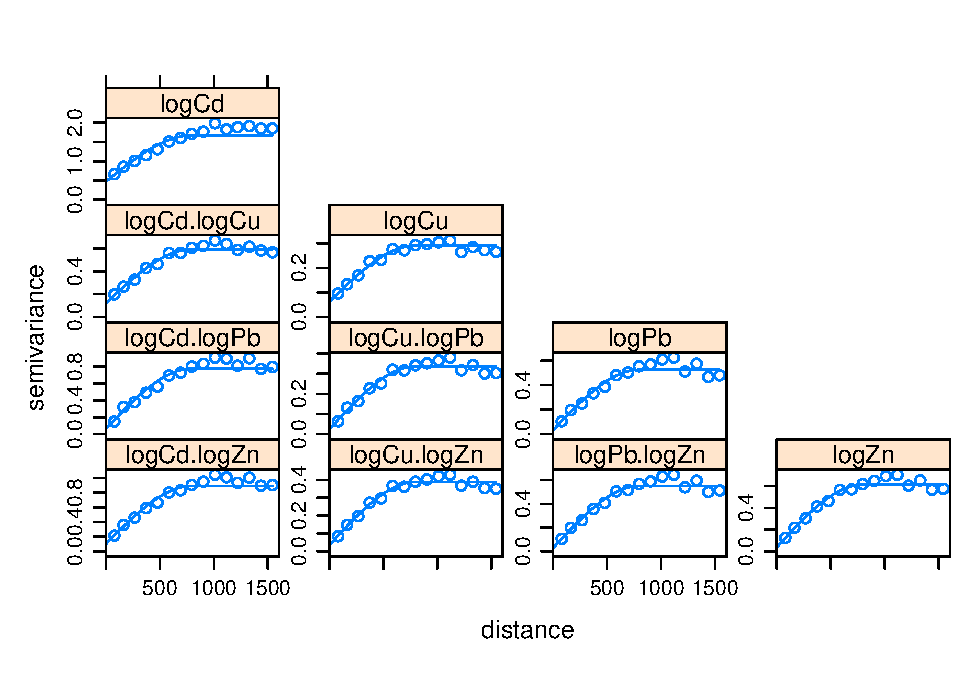
\includegraphics{_main_files/figure-latex/unnamed-chunk-9-1.pdf}

\begin{Shaded}
\begin{Highlighting}[]
\NormalTok{CK }\OtherTok{\textless{}{-}} \FunctionTok{predict}\NormalTok{(CK.fit, GridBAUs) }\CommentTok{\# Ordinary CoKriging}
\end{Highlighting}
\end{Shaded}

\begin{verbatim}
## Linear Model of Coregionalization found. Good.
## [using ordinary cokriging]
\end{verbatim}

\begin{enumerate}
\def\labelenumi{\arabic{enumi}.}
\setcounter{enumi}{4}
\tightlist
\item
  各種模型比較
\end{enumerate}

\begin{Shaded}
\begin{Highlighting}[]
\NormalTok{OK.plot }\OtherTok{\textless{}{-}}\NormalTok{ OK }\SpecialCharTok{\%\textgreater{}\%}\NormalTok{ as.data.frame }\SpecialCharTok{\%\textgreater{}\%}
  \FunctionTok{ggplot}\NormalTok{() }\SpecialCharTok{+} \FunctionTok{aes}\NormalTok{(x,y,}\AttributeTok{fill =}\NormalTok{ var1.pred) }\SpecialCharTok{+} 
  \FunctionTok{geom\_tile}\NormalTok{() }\SpecialCharTok{+} \FunctionTok{coord\_fixed}\NormalTok{() }\SpecialCharTok{+} \FunctionTok{theme\_bw}\NormalTok{() }\SpecialCharTok{+} \FunctionTok{labs}\NormalTok{(}\AttributeTok{title =} \StringTok{\textquotesingle{}Ordinary Kriging\textquotesingle{}}\NormalTok{) }\SpecialCharTok{+} 
  \FunctionTok{scale\_fill\_distiller}\NormalTok{(}\AttributeTok{palette=}\StringTok{"Spectral"}\NormalTok{, }\AttributeTok{name=}\StringTok{"pred."}\NormalTok{)  }\SpecialCharTok{+} 
  \FunctionTok{geom\_point}\NormalTok{(}\AttributeTok{data=}\FunctionTok{data.frame}\NormalTok{(meuse), }\FunctionTok{aes}\NormalTok{(x,y,}\AttributeTok{fill=}\FunctionTok{log}\NormalTok{(zinc)), }\AttributeTok{colour=}\StringTok{"black"}\NormalTok{,}
             \AttributeTok{pch=}\DecValTok{21}\NormalTok{, }\AttributeTok{size=}\DecValTok{3}\NormalTok{) }

\NormalTok{UK.plot }\OtherTok{\textless{}{-}}\NormalTok{ UK }\SpecialCharTok{\%\textgreater{}\%}\NormalTok{ as.data.frame }\SpecialCharTok{\%\textgreater{}\%}
  \FunctionTok{ggplot}\NormalTok{() }\SpecialCharTok{+} \FunctionTok{aes}\NormalTok{(x,y,}\AttributeTok{fill =}\NormalTok{ var1.pred) }\SpecialCharTok{+} 
  \FunctionTok{geom\_tile}\NormalTok{() }\SpecialCharTok{+} \FunctionTok{coord\_fixed}\NormalTok{() }\SpecialCharTok{+} \FunctionTok{theme\_bw}\NormalTok{() }\SpecialCharTok{+} \FunctionTok{labs}\NormalTok{(}\AttributeTok{title =} \StringTok{\textquotesingle{}Universal Kriging\textquotesingle{}}\NormalTok{) }\SpecialCharTok{+} 
  \FunctionTok{scale\_fill\_distiller}\NormalTok{(}\AttributeTok{palette=}\StringTok{"Spectral"}\NormalTok{, }\AttributeTok{name=}\StringTok{"pred."}\NormalTok{)  }\SpecialCharTok{+} 
  \FunctionTok{geom\_point}\NormalTok{(}\AttributeTok{data=}\FunctionTok{data.frame}\NormalTok{(meuse), }\FunctionTok{aes}\NormalTok{(x,y,}\AttributeTok{fill=}\FunctionTok{log}\NormalTok{(zinc)), }\AttributeTok{colour=}\StringTok{"black"}\NormalTok{,}
             \AttributeTok{pch=}\DecValTok{21}\NormalTok{, }\AttributeTok{size=}\DecValTok{3}\NormalTok{) }
 
\NormalTok{SK.plot }\OtherTok{\textless{}{-}}\NormalTok{ SK }\SpecialCharTok{\%\textgreater{}\%}\NormalTok{ as.data.frame }\SpecialCharTok{\%\textgreater{}\%}
  \FunctionTok{ggplot}\NormalTok{() }\SpecialCharTok{+} \FunctionTok{aes}\NormalTok{(x,y,}\AttributeTok{fill =}\NormalTok{ var1.pred) }\SpecialCharTok{+} 
  \FunctionTok{geom\_tile}\NormalTok{() }\SpecialCharTok{+} \FunctionTok{coord\_fixed}\NormalTok{() }\SpecialCharTok{+} \FunctionTok{theme\_bw}\NormalTok{() }\SpecialCharTok{+} \FunctionTok{labs}\NormalTok{(}\AttributeTok{title =} \StringTok{\textquotesingle{}Simple Kriging\textquotesingle{}}\NormalTok{) }\SpecialCharTok{+} 
  \FunctionTok{scale\_fill\_distiller}\NormalTok{(}\AttributeTok{palette=}\StringTok{"Spectral"}\NormalTok{, }\AttributeTok{name=}\StringTok{"pred."}\NormalTok{)  }\SpecialCharTok{+} 
  \FunctionTok{geom\_point}\NormalTok{(}\AttributeTok{data=}\FunctionTok{data.frame}\NormalTok{(meuse), }\FunctionTok{aes}\NormalTok{(x,y,}\AttributeTok{fill=}\FunctionTok{log}\NormalTok{(zinc)), }\AttributeTok{colour=}\StringTok{"black"}\NormalTok{,}
             \AttributeTok{pch=}\DecValTok{21}\NormalTok{, }\AttributeTok{size=}\DecValTok{3}\NormalTok{) }

\NormalTok{CK.plot }\OtherTok{\textless{}{-}}\NormalTok{ CK }\SpecialCharTok{\%\textgreater{}\%}\NormalTok{ as.data.frame }\SpecialCharTok{\%\textgreater{}\%}
  \FunctionTok{ggplot}\NormalTok{() }\SpecialCharTok{+} \FunctionTok{aes}\NormalTok{(x,y,}\AttributeTok{fill =}\NormalTok{ logZn.pred) }\SpecialCharTok{+} 
  \FunctionTok{geom\_tile}\NormalTok{() }\SpecialCharTok{+} \FunctionTok{coord\_fixed}\NormalTok{() }\SpecialCharTok{+} \FunctionTok{theme\_bw}\NormalTok{() }\SpecialCharTok{+} \FunctionTok{labs}\NormalTok{(}\AttributeTok{title =} \StringTok{\textquotesingle{}CoKriging\textquotesingle{}}\NormalTok{) }\SpecialCharTok{+} 
  \FunctionTok{scale\_fill\_distiller}\NormalTok{(}\AttributeTok{palette=}\StringTok{"Spectral"}\NormalTok{, }\AttributeTok{name=}\StringTok{"pred."}\NormalTok{)  }\SpecialCharTok{+} 
  \FunctionTok{geom\_point}\NormalTok{(}\AttributeTok{data=}\FunctionTok{data.frame}\NormalTok{(meuse), }\FunctionTok{aes}\NormalTok{(x,y,}\AttributeTok{fill=}\FunctionTok{log}\NormalTok{(zinc)), }\AttributeTok{colour=}\StringTok{"black"}\NormalTok{,}
             \AttributeTok{pch=}\DecValTok{21}\NormalTok{, }\AttributeTok{size=}\DecValTok{3}\NormalTok{)}
  
\FunctionTok{grid.arrange}\NormalTok{(SK.plot, OK.plot, UK.plot, CK.plot, }\AttributeTok{ncol =} \DecValTok{2}\NormalTok{)}
\end{Highlighting}
\end{Shaded}

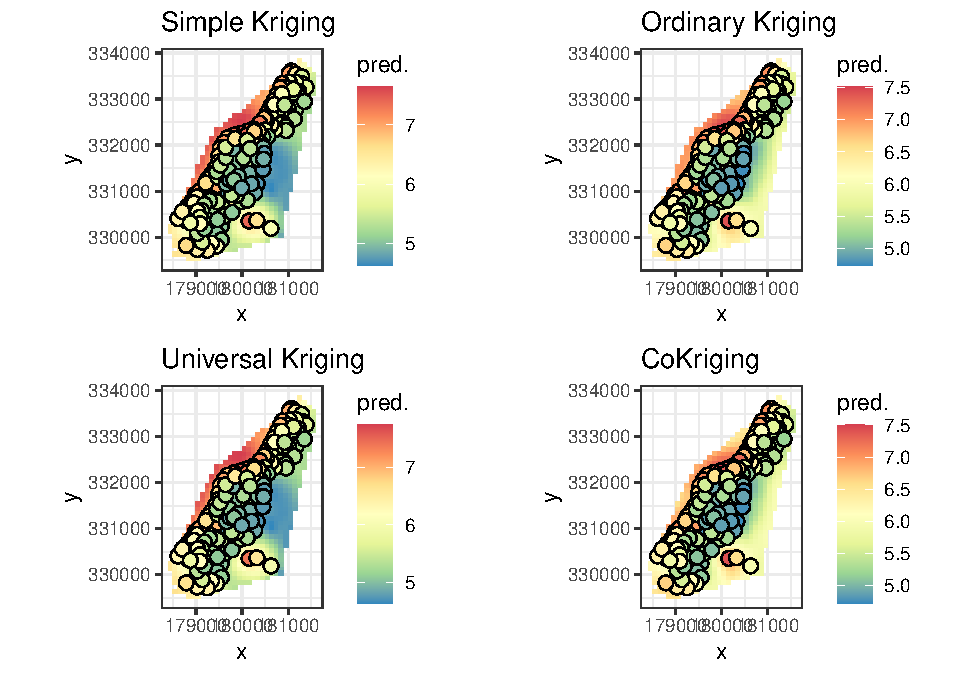
\includegraphics{_main_files/figure-latex/unnamed-chunk-10-1.pdf}

\begin{enumerate}
\def\labelenumi{\arabic{enumi}.}
\setcounter{enumi}{5}
\tightlist
\item
  比較各種模型誤差
\end{enumerate}

\begin{Shaded}
\begin{Highlighting}[]
\NormalTok{OK.varplot }\OtherTok{\textless{}{-}}\NormalTok{ OK }\SpecialCharTok{\%\textgreater{}\%}\NormalTok{ as.data.frame }\SpecialCharTok{\%\textgreater{}\%}
  \FunctionTok{ggplot}\NormalTok{() }\SpecialCharTok{+} \FunctionTok{aes}\NormalTok{(x,y,}\AttributeTok{fill =}\NormalTok{ var1.var) }\SpecialCharTok{+} 
  \FunctionTok{geom\_tile}\NormalTok{() }\SpecialCharTok{+} \FunctionTok{coord\_fixed}\NormalTok{() }\SpecialCharTok{+} \FunctionTok{theme\_bw}\NormalTok{() }\SpecialCharTok{+} \FunctionTok{labs}\NormalTok{(}\AttributeTok{title =} \StringTok{\textquotesingle{}Ordinary Kriging\textquotesingle{}}\NormalTok{) }\SpecialCharTok{+} 
  \FunctionTok{scale\_fill\_distiller}\NormalTok{(}\AttributeTok{palette=}\StringTok{"Spectral"}\NormalTok{, }\AttributeTok{name=}\StringTok{"var."}\NormalTok{)}

\NormalTok{UK.varplot }\OtherTok{\textless{}{-}}\NormalTok{ UK }\SpecialCharTok{\%\textgreater{}\%}\NormalTok{ as.data.frame }\SpecialCharTok{\%\textgreater{}\%}
  \FunctionTok{ggplot}\NormalTok{() }\SpecialCharTok{+} \FunctionTok{aes}\NormalTok{(x,y,}\AttributeTok{fill =}\NormalTok{ var1.var) }\SpecialCharTok{+} 
  \FunctionTok{geom\_tile}\NormalTok{() }\SpecialCharTok{+} \FunctionTok{coord\_fixed}\NormalTok{() }\SpecialCharTok{+} \FunctionTok{theme\_bw}\NormalTok{() }\SpecialCharTok{+} \FunctionTok{labs}\NormalTok{(}\AttributeTok{title =} \StringTok{\textquotesingle{}Universal Kriging\textquotesingle{}}\NormalTok{) }\SpecialCharTok{+} 
  \FunctionTok{scale\_fill\_distiller}\NormalTok{(}\AttributeTok{palette=}\StringTok{"Spectral"}\NormalTok{, }\AttributeTok{name=}\StringTok{"var."}\NormalTok{)}

\NormalTok{SK.varplot }\OtherTok{\textless{}{-}}\NormalTok{ SK }\SpecialCharTok{\%\textgreater{}\%}\NormalTok{ as.data.frame }\SpecialCharTok{\%\textgreater{}\%}
  \FunctionTok{ggplot}\NormalTok{() }\SpecialCharTok{+} \FunctionTok{aes}\NormalTok{(x,y,}\AttributeTok{fill =}\NormalTok{ var1.var) }\SpecialCharTok{+} 
  \FunctionTok{geom\_tile}\NormalTok{() }\SpecialCharTok{+} \FunctionTok{coord\_fixed}\NormalTok{() }\SpecialCharTok{+} \FunctionTok{theme\_bw}\NormalTok{() }\SpecialCharTok{+} \FunctionTok{labs}\NormalTok{(}\AttributeTok{title =} \StringTok{\textquotesingle{}Simple Kriging\textquotesingle{}}\NormalTok{) }\SpecialCharTok{+} 
  \FunctionTok{scale\_fill\_distiller}\NormalTok{(}\AttributeTok{palette=}\StringTok{"Spectral"}\NormalTok{, }\AttributeTok{name=}\StringTok{"var."}\NormalTok{)}

\NormalTok{CK.varplot }\OtherTok{\textless{}{-}}\NormalTok{ CK }\SpecialCharTok{\%\textgreater{}\%}\NormalTok{ as.data.frame }\SpecialCharTok{\%\textgreater{}\%}
  \FunctionTok{ggplot}\NormalTok{() }\SpecialCharTok{+} \FunctionTok{aes}\NormalTok{(x,y,}\AttributeTok{fill =}\NormalTok{ logZn.var) }\SpecialCharTok{+} 
  \FunctionTok{geom\_tile}\NormalTok{() }\SpecialCharTok{+} \FunctionTok{coord\_fixed}\NormalTok{() }\SpecialCharTok{+} \FunctionTok{theme\_bw}\NormalTok{() }\SpecialCharTok{+} \FunctionTok{labs}\NormalTok{(}\AttributeTok{title =} \StringTok{\textquotesingle{}CoKriging\textquotesingle{}}\NormalTok{) }\SpecialCharTok{+} 
  \FunctionTok{scale\_fill\_distiller}\NormalTok{(}\AttributeTok{palette=}\StringTok{"Spectral"}\NormalTok{, }\AttributeTok{name=}\StringTok{"var."}\NormalTok{)}
  
\FunctionTok{grid.arrange}\NormalTok{(SK.varplot, OK.varplot, UK.varplot, CK.varplot, }\AttributeTok{ncol =} \DecValTok{2}\NormalTok{)}
\end{Highlighting}
\end{Shaded}

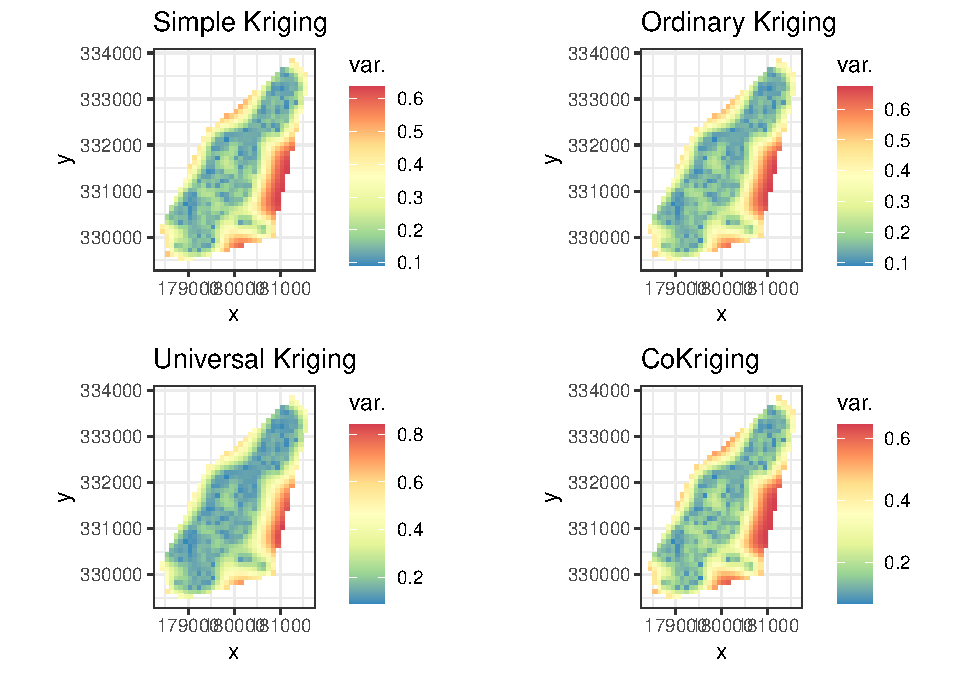
\includegraphics{_main_files/figure-latex/unnamed-chunk-11-1.pdf}

\begin{enumerate}
\def\labelenumi{\arabic{enumi}.}
\setcounter{enumi}{6}
\tightlist
\item
  克里金模型交叉驗證
\end{enumerate}

\begin{Shaded}
\begin{Highlighting}[]
\NormalTok{OK.cv }\OtherTok{\textless{}{-}} \FunctionTok{krige.cv}\NormalTok{(}\FunctionTok{log}\NormalTok{(zinc) }\SpecialCharTok{\textasciitilde{}} \DecValTok{1}\NormalTok{, meuse, lzn.fit,}
               \AttributeTok{nfold =} \DecValTok{10}\NormalTok{, }\AttributeTok{verbose =}\NormalTok{ F)}
\NormalTok{UK.cv }\OtherTok{\textless{}{-}} \FunctionTok{krige.cv}\NormalTok{(}\FunctionTok{log}\NormalTok{(zinc) }\SpecialCharTok{\textasciitilde{}}\NormalTok{ x }\SpecialCharTok{+}\NormalTok{ y, meuse, lzn.fit,}
                  \AttributeTok{nfold =} \DecValTok{10}\NormalTok{, }\AttributeTok{verbose =}\NormalTok{ F)}
\NormalTok{SK.cv }\OtherTok{\textless{}{-}} \FunctionTok{krige.cv}\NormalTok{(}\FunctionTok{log}\NormalTok{(zinc) }\SpecialCharTok{\textasciitilde{}}\NormalTok{ x }\SpecialCharTok{+}\NormalTok{ y, meuse, lzn.fit,}
                  \AttributeTok{nfold =} \DecValTok{10}\NormalTok{, }\AttributeTok{verbose =}\NormalTok{ F, }\AttributeTok{beta =} \FunctionTok{c}\NormalTok{(}\SpecialCharTok{{-}}\FloatTok{8.0324313}\NormalTok{, }\SpecialCharTok{{-}}\FloatTok{0.0008891}\NormalTok{, }\FloatTok{0.0005250}\NormalTok{))}
\NormalTok{CK.cv }\OtherTok{\textless{}{-}} \FunctionTok{gstat.cv}\NormalTok{(CK.fit, }\AttributeTok{verbose =}\NormalTok{ F, }\AttributeTok{all.residuals =}\NormalTok{ T)}
\end{Highlighting}
\end{Shaded}

\hypertarget{linear-algebra}{%
\chapter{Linear Algebra}\label{linear-algebra}}

\hypertarget{vector-space-ux5411ux91cfux7a7aux9593}{%
\section{Vector Space (向量空間)}\label{vector-space-ux5411ux91cfux7a7aux9593}}

令 \(V\) 為非空集合(元素為向量),\(F\) 為體(元素為純量)
滿足以下八條規則稱 \((V,+,\cdot)\) 為佈於 \(F\) 的向量空間 :

\begin{enumerate}
\def\labelenumi{\arabic{enumi}.}
\tightlist
\item
  向量加法結合律
  \(\forall\) \(u,v,w \in V\), \((u + v) + w = u + (v + w)\)
\item
  向量加法單位元素
  \(\exists\) \(0 \in V\) such that \(\forall\) \(v \in V\), we have \(v+0 = 0+v = v\)
\item
  向量加法反元素
  \(\forall\) \(v \in V\), \(\exists -v \in V\) such that \(v + (-v) = (-v) + v = 0\)
\item
  向量加法交換律
  \(\forall\) \(u,v \in V\), \(u+v = v+u\)
\item
  純量乘法對向量加法有分配律
  \(\forall\) \(\alpha \in F\), \(u,v \in V\), \(\alpha \cdot(u+v) = \alpha \cdot u + \alpha \cdot v\)
\item
  純量乘法對純量加法有分配律
  \(\forall\) \(\alpha, \beta \in F\), \(v \in V\), \((\alpha + \beta) \cdot v = \alpha \cdot v + \beta \cdot v\)
\item
  純量乘法結合律
  \(\forall\) \(\alpha, \beta \in F\), \(v \in V\), \((\alpha\beta) v = \alpha(\beta v)\)
\item
  乘法單位元素
  \(\forall v \in V\), \(1 \cdot v = v\)
\end{enumerate}

\textbf{Note :}
- 向量空間必有零向量(非空)

\hypertarget{subspacce-ux5b50ux7a7aux9593}{%
\subsection{Subspacce (子空間)}\label{subspacce-ux5b50ux7a7aux9593}}

令 \(S\) 為 \(V\) 的非空子集,且佈於同一 \(F\) 上,稱 \((S,+, \cdot)\) 為 \((V,+,\cdot)\) 的子空間

\textbf{Note} (令向量空間 \(W\) 為向量空間 \(V\) 的子空間) \textbf{:}

\begin{itemize}
\tightlist
\item
  \(\{0\}\), \(V\) 皆為向量空間 \(V\) 的顯然子空間(trivial subspace)
\item
  歐式空間的子空間必然通過原點
\item
  子空間有向量加法封閉性以及純量乘法封閉性

  \begin{itemize}
  \tightlist
  \item
    \(\forall\) \(u,v\in W\), \(\alpha \in F\), \(\alpha u +v \in W\)
  \end{itemize}
\item
  \(0 \in W\)        (常用來判斷是否為子空間)
\item
  if \(v\in W\), then \(-v \in W\) (常用來判斷是否為子空間)
\item
  子空間交集仍為子空間
\item
  子空間聯集為子空間,若且唯若子空間之間有包含關係
\end{itemize}

\hypertarget{sum-space-ux548cux7a7aux9593}{%
\subsection{Sum space (和空間)}\label{sum-space-ux548cux7a7aux9593}}

假設 \(W_1, \cdots, W_k\) 為 \(V\) 的子空間,則 \(\displaystyle \sum_{i = 1}^k W_i := \{\sum_{i=1}^kv_i|v_i \in W_i, 1 \leq i \leq k\}\) 稱為 \(W_1, \cdots, W_k\) 的和空間

\textbf{Note :}

\begin{itemize}
\tightlist
\item
  子空間的和空間仍為子空間
\item
  \(W_1\) \(\cup\) \(W_2\) \(\subseteq\) \(W_1 + W_2\)
\item
  \(W_1 + W_2\) 是包含 \(W_1\) \(\cup\) \(W_2\) 的最小子空間
\end{itemize}

\hypertarget{four-basis-spaces-ux56dbux5927ux57faux672cux5b50ux7a7aux9593}{%
\subsection{Four Basis Spaces (四大基本子空間)}\label{four-basis-spaces-ux56dbux5927ux57faux672cux5b50ux7a7aux9593}}

假設 \(A \in F^{m \times n}\)

\begin{enumerate}
\def\labelenumi{\arabic{enumi}.}
\tightlist
\item
  Row space 為 \(A\) row vector 的線性組合,\(\mbox{RS}(A) = \{xA|x\in F^{1 \times m}\}\)
\item
  Column space 為 \(A\) colume vector 的線性組合,\(\mbox{CS}(A) = \{Ax|x\in F^{m\times 1}\}\)
\item
  kernal space 為 \(Ax = 0\) 的 solution space,\(\mbox{ker}(A) = \{x \in F^{m \times 1}|Ax = 0\}\)
\item
  left kernal space 為 \(xA = 0\) 的 solution space,\(L\mbox{ker}(A) = \{x \in F^{1 \times m}|xA = 0\}\)
\end{enumerate}

\textbf{Note :}

\begin{enumerate}
\def\labelenumi{\arabic{enumi}.}
\tightlist
\item
  \(\mbox{CS}(A) = \mbox{Range}(A) = \mbox{R}(A)\)
\item
  \(\mbox{ker}(A) = \mbox{Nullspace}(A) = \mbox{Null(A)} = \mbox{N}(A)\)
\item
  \(L\mbox{ker}(A) = \mbox{ker}(A^T)\),(\(A\) 的 row vector 為 \(A^T\) 的 column vector)
\item
  列運算不改變 Row space 和 kernal space
  若\(A\) row equivalent to \(B\) 則 \(\mbox{RS}(A) = \mbox{RS}(B)\) 且 \(\mbox{ker}(A) = \mbox{ker}(B)\)
\item
  行運算不改變 Column space 和 left kernal space
  若\(A\) cloumn equivalent to \(B\) 則 \(\mbox{CS}(A) = \mbox{CS}(B)\) 且 \(L\mbox{ker}(A) = L\mbox{ker}(B)\)
\item
  \(\mbox{RS}(AB) \subseteq \mbox{RS}(B);\) \(\mbox{CS}(AB) \subseteq \mbox{CS}(A)\)
\item
  若 \(AB = O\) 則 \(\mbox{CS}(B)\subseteq \mbox{ker}(A);\) \(\mbox{RS}(A) \subseteq L\mbox{ker}(B)\)
\item
  \(Ax = b\) is consistent 若且唯若 \(b \in \mbox{CS}(A)\)
\end{enumerate}

\textbf{Clearly explaintion on feature 6. :}

\[A_{m \times n}B_{n \times m} = \begin{bmatrix}
 | & \vdots & | \\
 a_1 & \cdots & a_n \\
 | & \vdots & |
\end{bmatrix}\begin{bmatrix}
 b_{11} & \cdots & b_{1m}\\
 \vdots & \ddots & \vdots\\
 b_{n1} & \cdots & b_{nm}
\end{bmatrix}\]
\(AB\) 可以看做是 \(A\) Column vector 的線性組合,顯而易見地 \(AB\) 的 Column space 自然會包含於 \(A\) 的 Column space

\[
A_{m\times n}B_{n \times m} = \begin{bmatrix}
 a_{11} & \cdots & a_{1n}\\
 \vdots & \ddots & \vdots\\
 a_{m1} & \cdots & a_{mn}
\end{bmatrix}\begin{bmatrix}
 - & b_1 & -\\
 \cdots & \vdots & \cdots\\
 - & b_n &-
\end{bmatrix}
\]

\(AB\) 也可以看做是 \(B\) Row vector 的線性組合,顯而易見地 \(AB\) 的 Row space 自然會包含於 \(B\) 的 Row space

\textbf{Clearly explaintion on feature 7. :}

let \(y \in \mbox{CS}(B)\), i.e., \(y = Bx\) for some \(x\), then we have following relation \(AB = O \implies (AB)x = Ox = 0 \iff A(Bx) = 0 \iff Ay = 0 \iff y \in \mbox{ker}(A)\)

let \(y \in \mbox{RS}(A)\), i.e., \(y = xA\) for some \(x\), then we have following relation \(AB = O \implies x(AB) = xO = 0 \iff (xA)B = 0 \iff yB = 0 \iff y \in L\mbox{ker}(B)\)

\hypertarget{solve-linear-system-ux6c42ux89e3ux7ddaux6027ux7cfbux7d71}{%
\subsection{Solve Linear System (求解線性系統)}\label{solve-linear-system-ux6c42ux89e3ux7ddaux6027ux7cfbux7d71}}

令 \(A \in F^{m \times n}\) 且 \(x, b \in F^{1 \times n}\)

\begin{itemize}
\tightlist
\item
  線性系統 \(Ax = b\) 的其中一解稱為特解 (particular solution)
\item
  線性系統 \(Ax = 0\) 的解稱為零解 (homogeneous solution)
\item
  線性系統 \(Ax = b\) 的解為一個特解加上零解
\item
  A linear system \(Ax = b\) is called consistent if \(b \in \mbox{CS}(A)\)
\item
  A linear system \(Ax = b\) is called inconsistent if \(b \notin \mbox{CS}(A)\)
\end{itemize}

\hypertarget{ux7ddaux6027ux7cfbux7d71ux6c42ux89e3ux6f14ux7b97ux6cd5}{%
\subsection{線性系統求解演算法}\label{ux7ddaux6027ux7cfbux7d71ux6c42ux89e3ux6f14ux7b97ux6cd5}}

\begin{enumerate}
\def\labelenumi{\arabic{enumi}.}
\tightlist
\item
  \(\mbox{Input :}\) an consistent matrix \(A_{m \times n}\) and vector \(b\) which is in the column space of \(A\)
\item
  Do row operation to obtain the echlon form \((A\mid b) \rightarrow (R \mid r)\)
\item
  Find all the free variables \(y_1, \cdots, y_k\)
\item
  Set \(y_1= \cdots = y_k = 0\), solve \(Rx = r\) and get a particular solution \(p\)
\item
  For each \(i = 1, \cdots, k\) set \(y_i = 1\) and other \(y = 0\), solve \(Rx = 0\) and get a homogeneous solution \(\beta_i\)
\item
  \(\mbox{Output :}\) \(p + c_1\beta_1 + \cdots + c_k\beta_k\)
\end{enumerate}

\hypertarget{spanning-set-and-generating-set-ux751fux6210ux96c6ux8207ux7368ux7acbux96c6}{%
\subsection{Spanning Set and Generating Set (生成集與獨立集)}\label{spanning-set-and-generating-set-ux751fux6210ux96c6ux8207ux7368ux7acbux96c6}}

令 \(S\) 為向量空間 \(V_F\) 的子集合,\(\displaystyle span(S) = \{\sum_{i = 1}^{k}\alpha_i v_i \mid v_i \in S, \alpha_i \in F, 1 \leq i \leq k\}\) 稱為集合 \(S\) 的生成空間而 \(S\) 為\(span(S)\) 的生成集

\textbf{Note} (令 \(S,S_1,S_2\) 為向量空間 \(V_F\) 的子集合) \textbf{:}

\begin{itemize}
\tightlist
\item
  我們約定 \(span(\phi) = \{0\}\)
\item
  \(span(S)\) 滿足加法與存量乘法封閉性,為包含 \(S\) 的最小子空間
\item
  \(\mbox{RS}(A) = span(\{\mbox{all the row vector in A}\})\)
\item
  \(\mbox{CS}(A) = span(\{\mbox{all the column vector in A}\})\)
\item
  \(S \subseteq span(S)\) 且若 \(S_1 \subseteq S_2 \subseteq V\) 則 \(span(S_1) \subseteq span(S_2)\)
\item
  \(span(S_1)\) \(\cup\) \(span(S_2) \subseteq span(S_1\) \(\cup\) \(S_2)\)
\item
  \(span(S_1)\) \(\cap\) \(span(S_2) \supseteq span(S_1\) \(\cap\) \(S_2)\)
\item
  \(S\) 為 \(W\) 的子空間,則 \(span(S) \subseteq W\)
\end{itemize}

\hypertarget{ux548cux7a7aux9593ux7684ux751fux6210ux96c6}{%
\subsection{和空間的生成集}\label{ux548cux7a7aux9593ux7684ux751fux6210ux96c6}}

若 \(W_1 = span(S_1)\), \(W_2 = span(S_2)\),則\(W_1 + W_2 = span(S_1\) \(\cup\) \(S_2) = span(S_1) + span(S_2)\)

\textbf{Note :}

\begin{itemize}
\tightlist
\item
  求和空間時,就取個別生成集聯集
\end{itemize}

\hypertarget{linear-independent-and-linear-dependent-ux7ddaux6027ux7368ux7acbux8207ux7ddaux6027ux76f8ux4f9d}{%
\section{Linear independent and Linear dependent (線性獨立與線性相依)}\label{linear-independent-and-linear-dependent-ux7ddaux6027ux7368ux7acbux8207ux7ddaux6027ux76f8ux4f9d}}

假設 \(V_F\) 為向量空間且有子集 \(S\),給定有現向量 \(v_1,\cdots,v_k \in S\) 和純量 \(c_1,\cdots,c_k \in F\)

若 \(c_1v_1 + \cdots + c_kv_k = 0 \iff c_i \neq 0\) for some \(1\leq i \leq k\),則稱 \(S\) 為線性相依集
若 \(c_1v_1 + \cdots + c_kv_k = 0 \iff c_i = 0\) for all \(1\leq i \leq k\),則稱 \(S\) 為線性獨立集

\textbf{Note :}

\begin{itemize}
\tightlist
\item
  我們約定 \(\phi\) 為線性獨立集
\item
  向量空間的子集不是線性相依就是線性獨立
\item
  \(\{0\}\) 是線性相依集 \(\implies\) 所有含有 \(\{0\}\) 的子集向量必是線性相依集
\item
  若 \(S\) 為線性相依集,則表示 \(S\) 中的元素可以表示為其他元素線性組合
\item
  包含線性相依的子集必是線性相依,線性獨立集的子集必是線性獨立
\item
  \(\{v_1,\cdots,v_n\} \in \mathbb{R}^n\) 是線性獨立集,則 \(\{Av_1,\cdots,Av_n\} \in \mathbb{R}^n\) 是線性獨立集 \(\iff A\) 可逆
\end{itemize}

\hypertarget{ux7ddaux6027ux7368ux7acbux5224ux5225ux6cd5}{%
\subsection{線性獨立判別法}\label{ux7ddaux6027ux7368ux7acbux5224ux5225ux6cd5}}

\begin{enumerate}
\def\labelenumi{\arabic{enumi}.}
\tightlist
\item
  依照定義做驗證
\item
  以列向量的形式排成矩陣做列運算
\item
  \(\mbox{Wronskian}\) 線性獨立判別法 (多用在函數的向量空間判斷)
\end{enumerate}

設 \(f_1, \cdots, f_n \in C^{(n-1)}[a,b]\),\(f_1, \cdots, f_n\) 的 \(\mbox{Wromskian}\) 定義為

\[
W[f_1, \cdots, f_n](x) = \begin{vmatrix}
 f_1(x) & f_2(x) & \cdots & f_n(x)\\
 f_1^{\prime}(x) &  f_2^{\prime}(x) & \cdots &  f_n^{\prime}(x)\\
 \vdots & \vdots & \ddots & \vdots\\
  f_1^{(n-1)}(x) &  f_2^{(n-1)}(x) & \cdots &  f_n^{(n-1)}(x)
\end{vmatrix}
\]

如果存在 \(x_0 \in [a, b]\) such that \(W[f_1, \cdots, f_n](x) \neq 0\) , 則 \(f_1,\cdots,f_n\) 為線性獨立集

\hypertarget{basis-and-space-property-ux57faux5e95ux8207ux7a7aux9593ux7279ux6027}{%
\section{Basis and Space Property (基底與空間特性)}\label{basis-and-space-property-ux57faux5e95ux8207ux7a7aux9593ux7279ux6027}}

向量空間 \(V_F\) 的子集 \(S\) 如果滿足 \(span(S) = V\) 和 \(S\) 為獨立集,則稱 \(S\) 為 \(V\) 的一組基底
向量空間的維度被定義為基底的基數 (the dimension of vector space is the cardinality of a basis)

\textbf{Note :}

\begin{itemize}
\tightlist
\item
  我們約定 \(\{0\}\) 的基底是 \(\phi\)
\item
  一個不為獨立集的生成集必可移除一些向量使其成為一組基底
\item
  一個不為生成集的獨立集必可添加一些向量使其成為一組基底
\item
  \(S\) 為 \(V\) 的基底 \(\iff\) \(S\) 是 \(V\) 的最小生成集 \(\iff\) \(S\) 是 \(V\) 的最大獨立集
\item
  \(\{v_1,\cdots,v_n\} \in \mathbb{R}^n\) 是一組基底,則 \(\{Av_1,\cdots,Av_n\} \in \mathbb{R}^n\) 是一組基底 \(\iff A\) 可逆
\end{itemize}

\hypertarget{ux56dbux5927ux5b50ux7a7aux9593ux7684ux57faux5e95}{%
\subsection{四大子空間的基底}\label{ux56dbux5927ux5b50ux7a7aux9593ux7684ux57faux5e95}}

求 \(A\) 四大子空間基底,先做列運算 \(A \rightarrow R\),則我們有

\begin{enumerate}
\def\labelenumi{\arabic{enumi}.}
\tightlist
\item
  nonzero row vectors of \(R\) form a basis of \(\mbox{RS}(A)\)
\item
  the pivot of \(R\) corresponse to column vectors of \(A\) form a basis of \(\mbox{CS}(A)\)
\item
  \(\mbox{ker}(A) = \mbox{ker}(R)\) , therefore the basis of \(\mbox{ker}(R)\) form a basis of \(\mbox{ker}(A)\)
\item
  \(L\mbox{ker}(A) = \mbox{RS}(A)^{\bot}\) , therefore the vectors which perpendecular to the vectors in \(\mbox{RS}(A)\) form a basis of \(L\mbox{ker}(A)\)
\item
  if \(A = PR\) and \(\mbox{rank}(A) = r\) , \(P\) is invertible, then exactly \(r\) column vectors from mostleft form a basis of \(\mbox{CS}(A)\)
\end{enumerate}

\textbf{Note :}

\begin{itemize}
\tightlist
\item
  \(A = PR\) means that \(A\) is row equivalent to \(R\) and the procedure are represented by matrix \(P\)
\end{itemize}

\hypertarget{dimension-of-sum-space-ux548cux7a7aux9593ux7dadux5ea6}{%
\subsubsection{Dimension of Sum Space (和空間維度)}\label{dimension-of-sum-space-ux548cux7a7aux9593ux7dadux5ea6}}

\(\mbox{dim}(V) < \infty\),且 \(W_1\), \(W_2\subseteq V_F\) ,則 \(\mbox{dim}(W_1 + W_2) = \mbox{dim}(W_1) + \mbox{dim}(W_2) - \mbox{dim}(W_1\) \(\cap\) \(W_2)\)

\textbf{Note :}

\begin{itemize}
\tightlist
\item
  \(\mbox{dim}(W_1 + W_2) = \mbox{dim}(W_1) + \mbox{dim}(W_2) \iff W_1\) \(\cap\) \(W_2 = \{0\}\)
\item
  和空間維度公式不適用於排容原理
\end{itemize}

\hypertarget{linear-transformation-ux7ddaux6027ux6620ux5c04}{%
\section{Linear transformation (線性映射)}\label{linear-transformation-ux7ddaux6027ux6620ux5c04}}

在佈於 \(F\) 上的向量空間 \(V\) , \(W\),若函數 \(T:V \rightarrow W\) 滿足 \(\forall\) \(u, v \in V\) , \(c \in F\) 有
\(T(u+cv) = T(u) + cT(v)\),則稱 \(T\) 為從 \(V\) 到 \(W\) 的線性映射,寫作 \(T \in L(V, W)\)

令 \(X,Y\) 為 \(V,W\) 的子集
\(T(X) = \{T(v)\mid v \in X\}\) 稱為 \(X\) 之於 \(T\) 的像 (image)
\(T^{-1}(Y) = \{v \in V\mid T(v) \in Y\}\) 稱為 \(Y\) 之於 \(T\) 的反像 (preimage)

\textbf{Note :}

\begin{itemize}
\tightlist
\item
  \(T(0) = 0\) 且 \(T^{-1}\) 並非 \(T\) 的反函數
\item
  微分運算與積分運算為線性映射且有不可逆的矩陣表示法
\item
  若 \(T,U \in L(V,W)\),則 \(T = U \iff T(b_i) = U(b_i)\) 其中 \(b_i\) , \(1 \leq i \leq n\) 形成 \(V\) 的一組基底
\item
  對於同一個有序基底,線性變換存在唯一的矩陣表示法
\end{itemize}

\hypertarget{rank-of-a-matrix-ux77e9ux9663ux7684ux79e9}{%
\section{Rank of a Matrix (矩陣的秩)}\label{rank-of-a-matrix-ux77e9ux9663ux7684ux79e9}}

對於任意矩陣 \(A\) , \(\mbox{dim}(\mbox{RS}(A))\) 稱為 row rank of \(A\)
對於任意矩陣 \(A\) , \(\mbox{dim}(\mbox{CS}(A))\) 稱為 column rank of \(A\)

The definition of the rank of a matrix \(A\) is the dimension of Vector space spanned by the columns of \(A\), or the dimension of Vector space spanned by the row of \(A\), equivalently,

\(\mbox{rank} = \mbox{dim}(\mbox{RS}(A)) = \mbox{dim}(\mbox{CS}(A))\)  (詳見如何找四大空間基底)

\textbf{Note :}

\begin{itemize}
\tightlist
\item
  矩陣的秩可以看做可控參數的數目,而核空間的維度可以看做自由參數的數目 (參考自由度)
\item
  \(A \in F^{n \times n}\) 可逆 \(\iff\) \(A\) 是滿秩的 (full rank and \(\mbox{rank}(A) = n\))
\end{itemize}

\hypertarget{sylvester-theorem-ux79e9-ux96f6ux5ea6ux5b9aux7406}{%
\subsection{Sylvester Theorem (秩 零度定理)}\label{sylvester-theorem-ux79e9-ux96f6ux5ea6ux5b9aux7406}}

假設線性變換 \(T \in L(V,W)\) 有矩陣表示法 \(A \in F^{m \times n}\) 且 \(\mbox{dim}(V) < \infty\),則以下數學式常用

\begin{enumerate}
\def\labelenumi{\arabic{enumi}.}
\tightlist
\item
  \(n = nullity(A) + \mbox{rank}(A)\)
\item
  \(m = nullity(A^T) + \mbox{rank}(A^T) = nullity(A^T) + \mbox{rank}(A)\)
\item
  \(\mbox{dim}(V) = nullity(T) + \mbox{rank}(T)\)
\item
  \(V = \mbox{ker}(T) + \mbox{Im}(T) \iff \mbox{ker}(T)\) \(\cap\) \(\mbox{Im}(T) = \{0\}\)
\end{enumerate}

\hypertarget{property-of-the-rank-ux79e9ux7684ux7279ux6027}{%
\subsection{Property of the Rank (秩的特性)}\label{property-of-the-rank-ux79e9ux7684ux7279ux6027}}

\begin{enumerate}
\def\labelenumi{\arabic{enumi}.}
\tightlist
\item
  \(\mbox{rank}(A) = \mbox{rank}(A^T)\)
\item
  \(\mbox{rank}(A) \leq \min\{m,n\}\)
\item
  If \(A\) is row / column equivalent to \(R\) then \(\mbox{rank}(A) = \mbox{rank}(B)\)
\item
  \(\mbox{rank}(AB) \leq \min \{\mbox{rank}(A), \mbox{rank}(B)\}\)
\item
  若方陣 \(P\) 可逆,則 \(\mbox{rank}(PA) = \mbox{rank}(A)\) , \(\mbox{rank}(AP) = \mbox{rank}(A)\)
\item
  \(\mbox{rank}(A+ B) \leq \mbox{rank}(A) + \mbox{rank}(B)\)
\item
  \(Ax = b\) is consistent \(\iff\) \(\mbox{rank}([A \mid b]) = \mbox{rank}(A)\)
\item
  \(\forall\) \(b \in \mathbb{R}^{m \times 1}\) , \(Ax = b\) is consistent \(\iff \mbox{rank}(A) = m\)
  \(m=n \implies\) exactly one solution
  \(m < n \implies\) infinty solutions
\end{enumerate}

\textbf{Clearly explaintion :}

\begin{enumerate}
\def\labelenumi{\arabic{enumi}.}
\tightlist
\item
  矩陣的轉置會把 Column space 和 Row space 對調,並不影響他們的基底,故秩相同
\item
  Column space 和 Row space 的維度相同,故矩陣秩最大只能到\(\min \{\mbox{dimension of Column / Row space}\}\)
\item
  行列運算並不改變 Column space 和 Row sapce,故秩相同
\item
  \(AB\) 可以看做 \(A\) column vectors 的線性組合或 \(B\) row vectors 的線性組合,故 \(AB\) 的秩較小
\item
  \(PA\) 中的 \(P\) 可以看做基本列運算,故 \(A\) is row equivalent to \(PA\),故秩相同,同理可得後者
\item
  矩陣的秩可以看做可控參數的數目,故分別可控的數量必比和空間要多 (\(A\) 中可能存在某些向量與 \(B\) 中的向量線性相依)
\item
  增廣矩陣秩不變表示 \(b\) 為 \(A\) 中 column vectors 的線性組合,也就是說 \(b \in \mbox{CS}(A)\)
\item
  由秩零度定理知,\(nullity(A) > 0\),自由參數大於 \(1\) ,故無限多組解
\end{enumerate}

\hypertarget{direct-sum-and-projection-ux76f4ux548cux8207ux6295ux5f71}{%
\section{Direct Sum and Projection (直和與投影)}\label{direct-sum-and-projection-ux76f4ux548cux8207ux6295ux5f71}}

對於向量空間 \(V_F\) 與子空間 \(W_1, \cdots, W_k\),若 \(W_i\) \(\cap\) \(\displaystyle\sum_{i\neq j}W_j = \{0\}\) where \(1\leq i \leq k\) 則稱 \(W_1, \cdots, W_k\) 為獨自子空間,且若有 \(V = \displaystyle \sum_{i=1}^kW_i\),則稱 \(W_1, \cdots, W_k\) 為 \(V\) 的一個直和,記做 \(V = W_1 \oplus W_2 \cdots \oplus W_k\)

\textbf{Note :}

\begin{itemize}
\tightlist
\item
  對於任意 \(v \in V\) 存在唯一方式分解成 \(\sum w_i\) for \(1\leq i\leq k\) 其中 \(w_i \in W_i\)
\item
  任何一個\textbf{方陣}必可分解成一個對稱矩陣加上一個反對稱矩陣
\item
  任何一個\textbf{實函數}必可分解成一個奇函數加上一個偶函數
\end{itemize}

\hypertarget{projection-matrix-ux6295ux5f71ux77e9ux9663}{%
\subsection{Projection Matrix (投影矩陣)}\label{projection-matrix-ux6295ux5f71ux77e9ux9663}}

若 \(T \in L(V,V)\) 滿足 \(T^2 = T\) 則稱 \(T\) 為 \(V\) 上的投影/冪等算子 (projection / idempotent operator)
若 \(A \in F^{m\times n}\) 滿足 \(A^2 = A\) 則稱 \(A\) 為投影/冪等矩陣 (projection / idempotent matrix)

\textbf{Note :}

\begin{enumerate}
\def\labelenumi{\arabic{enumi}.}
\tightlist
\item
  投影矩陣投影兩次等於投影一次
\item
  投影矩陣把被投影的向量投影到該矩陣的 Column space 上
\item
  \(I_n - \frac{1}{n}J_n\) 為投影矩陣
\item
  若 \(A,B\) 皆為對稱矩陣,且滿足 \(AB\) 為投影矩陣,則 \(BA\) 為投影矩陣
\item
  若 \(A\) 為投影矩陣,則 \(I - A\) 也是投影矩陣
\item
  若方陣 \(A\) 為投影矩陣,則 \(A = I\) 或 \(A\) 不可逆
\end{enumerate}

\textbf{Clearly explaintion :}

\begin{enumerate}
\def\labelenumi{\arabic{enumi}.}
\tightlist
\item
  把向量 \(x\) 投影到 \(A\) 的 Coumn space 上後,\(x \in \mbox{CS}(A)\),在投影一次也是一樣的結果
\item
  \(Ax\) 代表 \(A\) column vectors 的線性組合,自然投影到 \(\mbox{CS}(A)\) 上,且投影兩次結果不變
\item
  \((I_n - \frac{1}{n}J_n)^2 = I_n - \frac{2}{n}J_n + \frac{1}{n^2}J_n^2 = I_n - \frac{1}{n}J_n\)
\item
  \((BA)^2 = ((A^TB^T)^T)^2 = ((AB)^T)^2 = ((AB)^2)^T = (AB)^T = BA\)
\item
  投影矩陣把向量投影到不同的獨立子空間後,根據直和的定義,他在各個獨立子空間有唯一分解表達式,故把表達式加總後會回到原來的向量,也就是說 \(I_n = (I_n - A) \oplus A\) 為投影矩陣 (詳見譜分解定理)
\item
  如果投影矩陣把原空間投影到相同的空間,則投影矩陣為單位矩陣
  如果投影矩陣把原空間投影到更低的維度時,他必然捨棄一些維度,故 \(A\) 不可逆
\end{enumerate}

\hypertarget{orthogonal-projection-ux6b63ux4ea4ux6295ux5f71}{%
\subsection{Orthogonal Projection (正交投影)}\label{orthogonal-projection-ux6b63ux4ea4ux6295ux5f71}}

若 \(V = X\oplus Y\), 根據直和定義 \(\forall \ z \in V\) \(z =x + y\) 其中 \(x \in X\) , \(y \in Y\),且線性算子 \(T(z) = x\),則稱線性算子 \(T\) 為沿著 \(Y\) 在 \(X\) 上的投影,更進一步,若 \(X\) 正交於 \(Y\),則稱為正交投影

\textbf{Example :} 在 \(\mathbb{R}^3\) 中,\(\mathbb{R}^3 = P \oplus L\),其中 \(P\) 為一平面,\(L\) 為一條直線,且 \(L\) 不在 \(P\) 上,則任何向量 \(z \in \mathbb{R}^3\) 皆可表示為 \(P\) 上的點和 \(P\) 外的點的和,而 \(P\) 上的點為 \(P\) 外的點沿著 \(L\) 在 \(P\) 上的投影

\hypertarget{change-basis-and-coordinates-matrix-ux57faux5e95ux8b8aux63dbux8207ux57faux5e95ux8b8aux63dbux77e9ux9663}{%
\section{Change Basis and Coordinates Matrix (基底變換與基底變換矩陣)}\label{change-basis-and-coordinates-matrix-ux57faux5e95ux8b8aux63dbux8207ux57faux5e95ux8b8aux63dbux77e9ux9663}}

假設 \(\beta = \{b_1 ,\cdots ,b_n\}\) 為向量空間 \(V\) 的一組有序基底,則任何一個向量 \(v \in V\) 可以用 \(\beta\) 中的基底表示,有 \(v = c_1b_1 + \cdots + c_nb_n\),且是唯一表示,記做 \(\begin{bmatrix}v\end{bmatrix}_{\beta}\)

假設有另外一組有序基底 \(\alpha = \{a_1,\cdots,a_n\}\),令矩陣 \(A, B\) 的 Column vector 分別由 \(\alpha, \beta\) 表示,
定義 \(\alpha\) 到 \(\beta\) 的基底變換矩陣為 \(P = [\ [a_1]_{\beta}, \cdots, [a_n]_{\beta}\ ]\) 其 Colmn vector 為 \(A\) 的 Column vector 在 \(\beta\) 基底下的表示法係數,且有以下關係 :

\begin{enumerate}
\def\labelenumi{\arabic{enumi}.}
\tightlist
\item
  \(\forall\ v \in V\) , \(\begin{bmatrix}v\end{bmatrix} _{\beta} = P\begin{bmatrix}v\end{bmatrix}_{\alpha}\)
\item
  \(BP = A\) or equivalently \(P = B^{-1}A\)
\end{enumerate}

\textbf{Clearly explaintion :}

\begin{enumerate}
\def\labelenumi{\arabic{enumi}.}
\tightlist
\item
  \(\begin{bmatrix}v\end{bmatrix}_{\alpha}\) 為在 \(\alpha\) 基底下的表示係數,而矩陣 \(P\) 為 \(\alpha\) 基底在 \(\beta\) 基底下的表示係數
\item
  考慮 \(BPv = Av\), \(Av\) 為 \(\alpha\) 中基底的線性組合,即用 \(\alpha\) 基底來看向量 \(v\)
  \(BPv\) 為 \(\beta\) 中基底的線性組合,即用 \(\beta\) 基底來看向量 \(v\),故兩者相同
\end{enumerate}

\hypertarget{ux7ddaux6027ux8b8aux63dbux77e9ux9663ux8868ux793aux6cd5}{%
\section{線性變換矩陣表示法}\label{ux7ddaux6027ux8b8aux63dbux77e9ux9663ux8868ux793aux6cd5}}

求性線變換 \(T \in L(V,V)\) 相對於 \(\alpha\) 的矩陣 \(A\) 表示法,先看基於哪一組基底 \((\alpha)\) (一般為標準正交基) ,將基底帶入線性算子中即為 \(A\) 的 Column vector,再用 \(\alpha\),記做 \(\begin{bmatrix}T\end{bmatrix}_{\alpha}\)

\[
A = \begin{bmatrix}
\mid &  & \mid \\
[T(a_1)]_{\alpha} & \cdots & [T(a_n)]_{\alpha} \\
\mid &  & \mid
\end{bmatrix}
\]

求性線變換 \(T \in L(V,W)\) 相對於 \(\alpha\) 到 \(\beta\) 的矩陣 \(A\) 表示法,先看基於哪一組基底 \((\alpha)\) (一般為標準正交基) ,將基底帶入線性算子中再用 \(\beta\) 的基底表示,即為 \(A\) 的 Column vector,記做 \(\begin{bmatrix}T\end{bmatrix}_{\alpha}^{\beta}\)

\[
A = \begin{bmatrix}
\mid &  & \mid \\
\begin{bmatrix}T(a_1)\end{bmatrix}_{\beta} & \cdots & \begin{bmatrix}T(a_n)\end{bmatrix}_{\beta} \\
\mid &  & \mid
\end{bmatrix}
\]

\textbf{Note :} (這裡假設 \(T\in L(V,W)\) 且 \(\alpha, \gamma\) 為 \(V\) 的一組基底 \(\beta, \gamma'\) 為 \(W\) 的一組基底)

\begin{enumerate}
\def\labelenumi{\arabic{enumi}.}
\tightlist
\item
  \(\forall\ v \in V\) , \(\begin{bmatrix}T(v)\end{bmatrix} _{\beta} = \begin{bmatrix}T\end{bmatrix}_{\alpha}^{\beta}\begin{bmatrix}v\end{bmatrix}_{\alpha}\)
\item
  \(\begin{bmatrix}T\end{bmatrix}_{\alpha}^{\beta} = \begin{bmatrix}I\end{bmatrix}_{\gamma'}^{\beta}\begin{bmatrix}T\end{bmatrix}_{\gamma}^{\gamma'}\begin{bmatrix}I\end{bmatrix}_{\alpha}^{\gamma}\)
\end{enumerate}

\hypertarget{similarity-of-the-square-matrix-ux65b9ux9663ux7684ux76f8ux4f3c}{%
\subsection{Similarity of the Square Matrix (方陣的相似)}\label{similarity-of-the-square-matrix-ux65b9ux9663ux7684ux76f8ux4f3c}}

考慮方陣 \(A, B\) 若存在 可逆矩陣 \(P\) 滿足 \(B = P^{-1}AP\) 則稱 \(A\) 與 \(B\) 相似 記做 \(A\) \(\sim\) \(B\)

\textbf{Note :} (假設 \(A \sim B\) )

\begin{enumerate}
\def\labelenumi{\arabic{enumi}.}
\tightlist
\item
  方陣的相似性為等價關係
\item
  \(I\) 只與 \(I\) 相似, \(O\) 只與 \(O\) 相似
\item
  同一個線性變換在不同基底之下的矩陣表示法相似
\item
  \(A^T \sim B^T\) 和 \(A^k \sim B^k\)
\item
  \(A + cI \sim B + cI\)
\item
  \(f(A) \sim f(B)\) 其中 \(f\) 為多項式函數
\item
  若 \(A, B\) 可逆,則 \(A^{-1} \sim B^{-1}\)
\item
  \(\mbox{tr}(A) = \mbox{tr}(B)\)
\item
  \(\mbox{det}(A) = \mbox{det}(B)\)
\item
  \(\mbox{rank}(A) = \mbox{rank}(B)\) 且 \(nullity(A) = nullity(B)\)
\end{enumerate}

反過來說,以上一項不成立,則 \(A \not\sim B\)

\hypertarget{eigenvalue-and-eigenvetor-ux7279ux5fb5ux503cux8207ux7279ux5fb5ux5411ux91cf}{%
\section{Eigenvalue and Eigenvetor (特徵值與特徵向量)}\label{eigenvalue-and-eigenvetor-ux7279ux5fb5ux503cux8207ux7279ux5fb5ux5411ux91cf}}

對於矩陣 \(A \in F^{n \times n}\),若存在 \(\lambda \in \mathbb{R}\) 和\textbf{非零}向量 \(v \in F^{n\times 1}\),使得 \(Av = \lambda v\),則稱 \(\lambda\) 為矩陣 \(A\) 的特徵值,\(v\) 為矩陣 \(A\) 的特徵向量

\textbf{Note :}

\begin{enumerate}
\def\labelenumi{\arabic{enumi}.}
\tightlist
\item
  \(\lambda\) 為矩陣 \(A\) 的特徵值 \(\iff \mbox{det}(A - \lambda I) = 0\)
\item
  \(\mbox{ker}(A)\) 中的非零向量均為特徵值 \(0\) 對應的特徵向量
\item
  若 \(v_1, v_2\) 為相對於 \(\lambda\) 的特徵向量,則 \(v_1 +v_2\) \((\neq 0)\) 亦為相對於 \(\lambda\) 的特徵向量
\item
  並非每個矩陣都有特徵值
\item
  若 \(A \sim B\),則 \(A\) 和 \(B\) 有相同特徵值與相對應的特徵向量 \(v, P^{-1}v\)
\item
  \(AB\) 和 \(BA\) 有相同特徵值
\item
  \(A\) 和 \(A^T\) 有相同特徵值
\item
  若 \(A\) 的各行(列)元素和均為 \(c\),則必有特徵值 \(c\)
\item
  \(A\) 可逆 \(\iff\) \(0\) 不為 \(A\) 的一個特徵值
\item
  如果 \(\lambda\) 是 \(A\) 相對於 \(v\) 的特徵值,則
  \(\frac{1}{\lambda}\) 為 \(A^{-1}\) 相對於 \(v\) 的特徵值
  \(\lambda^k\) 為 \(A^k\) 相對於 \(v\) 的特徵值
  \(f(\lambda)\) 為 \(f(A)\) 相對於 \(v\) 的特徵值,其中 \(f\) 為多項式函數
\end{enumerate}

\hypertarget{characteristic-polynomial-ux7279ux5fb5ux591aux9805ux5f0f}{%
\subsection{characteristic polynomial (特徵多項式)}\label{characteristic-polynomial-ux7279ux5fb5ux591aux9805ux5f0f}}

假設 \(A \in F^{n\times n}\),則特徵多項式被定義為 \(char_A(\lambda) = \mbox{det}(A - \lambda I)\),即解特徵值的方程式

\textbf{Note :}

\begin{enumerate}
\def\labelenumi{\arabic{enumi}.}
\tightlist
\item
  若 \(A \sim B\),則 \(char_A(\lambda) = char_B(\lambda)\)
\item
  \(A, B \in F^{n \times n}\),則 \(char_{AB}(\lambda) = char_{BA}(\lambda)\)
\item
  \(char_A(\lambda) = (-\lambda)^n + tr_1(A)(-\lambda)^{n-1} + \cdots + tr_{n-1}(A)(-\lambda) + tr_n(A)\),其中 \(tr_i(A)\) 為 \(A\) 中所有恰含 \(i\) 的對角項的 \(i\) 階子行列式的和
\item
  若 \(A\) 有特徵值 \(\lambda_1,\cdots, \lambda_k\),則 \(\lambda_1 + \cdots + \lambda_k = \mbox{tr}(A)\),\(\lambda_1\lambda_2\cdots \lambda_k = \mbox{det}(A)\)
\end{enumerate}

\hypertarget{eigenspace-and-multiplicity-ux7279ux5fb5ux7a7aux9593ux548cux91cdux6578}{%
\subsection{Eigenspace and multiplicity (特徵空間和重數)}\label{eigenspace-and-multiplicity-ux7279ux5fb5ux7a7aux9593ux548cux91cdux6578}}

假設 \(A \in F^{n\times n}\),\(v \in F^{n\times 1}\) 為 \(A\) 的特徵向量,定義 \(E_{\lambda_i} = \{v \mid Av = \lambda_i v,\lambda_i \in \mathbb{R}\} = \mbox{ker}(A - \lambda I)\) 為 \(\lambda_i\) 的特徵空間

代數重數為特徵值 \(\lambda_i\) 的重根個數,記做 \(am(\lambda_i)\)
幾何重數為特徵空間 \(E_{\lambda_i}\) 的維度,記做 \(gm(\lambda_i)\)

\textbf{Note :}

\begin{enumerate}
\def\labelenumi{\arabic{enumi}.}
\tightlist
\item
  \(\lambda\) 對應的特徵向量為 \(E_{\lambda_i}\) 中的非零向量
\item
  \(\lambda_1,\cdots,\lambda_k\) 為相異特徵值,則 \(E_{\lambda_1},\cdots,E_{\lambda_k}\) 為獨立子空間
\item
  \(gm(\lambda) = \mbox{dim}(E_{\lambda}) = nullity(T - \lambda I) = n - \mbox{rank}(T - \lambda I)\)
\item
  \(gm(0) = \mbox{dim}(E_0) = nullity(T) = n - \mbox{rank}(A)\)
\item
  \(1 \leq gm(\lambda) \leq am(\lambda) \leq n\)
\item
  若 \(\mbox{rank}(A) = k\),則 \(A\) 的相異特徵值最多 \(k\) 個
\end{enumerate}

\hypertarget{diagonalizable-ux53efux5c0dux89d2ux5316}{%
\section{Diagonalizable (可對角化)}\label{diagonalizable-ux53efux5c0dux89d2ux5316}}

假設 \(A \in F^{n\times n}\),若存在可逆矩陣 \(P\) 使得 \(P^{-1}AP = D\),其中 \(D\) 為對角矩陣,則稱 \(A\) 可對角化,即 \(A \sim D\)

\textbf{Clearly explantion on diagonalizable:}

矩陣對角化的精神在於用特徵向量當作基底,來表達任何一個在 \(V\) 中的向量,換句話說,如果特徵向量為 \(V\) 的生成集,則 \(v \in V\) 必可表示為特徵向量之和,過程如下 :

\textbf{Input :} a square matrix \(A\)

\begin{enumerate}
\def\labelenumi{\arabic{enumi}.}
\tightlist
\item
  Compute the characteristic polynomial \(char_A(\lambda) = \mbox{det}(A - \lambda I)\)
\item
  Factor \(char_A(\lambda) = (\lambda - \lambda_1)^{m1}(\lambda - \lambda_2)^{m2}\cdots(\lambda - \lambda_k)^{mk}\)
\item
  For each \(\lambda_i\) , compute a basis of \(E_{\lambda_i} = \mbox{ker}(A - \lambda_i I)\) and let \(d_i = \mbox{dim}(E_{\lambda_i})\)
\item
  If \(d_i = m_i\) for \(i = 1,\cdots,k\) then go to \(5.\)
  If \(d_i \neq m_i\) for some \(i\) , then not diagonalizable
\item
  \[D = \begin{bmatrix} \lambda_1 & \cdots & 0 \\ \vdots & \ddots & \vdots \\ 0 & \cdots & \lambda_k\end{bmatrix} \mbox{and}\ P = \begin{bmatrix}\mid & & \mid \\ v_1 & \cdots & v_k \\ \mid & & \mid\end{bmatrix} \ \mbox{where $v_i$ are the eigenbasis of $E_{\lambda_i}$}\]
\item
  \(A = PDP^{-1}\) or \(D = P^{-1}AP\)
\end{enumerate}

\textbf{Note :}

\begin{enumerate}
\def\labelenumi{\arabic{enumi}.}
\tightlist
\item
  \(A \in F^{n\times n}\) 可對角化 \(\iff A\) 有 \(n\) 個線性獨立的特徵向量
\item
  \(A \in F^{n\times n}\) 有 \(n\) 個相異的特徵值,則 \(A\) 有 \(n\) 個相互獨立的特徵向量
\item
  若 \(A\) 可對角化,則 \(A^T, A^{-1}, A^k, f(A)\) 皆可對角化,其中 \(f\) 為多項式函數
\item
  \(A\) 可否對角化與可逆無關 ( \(O\) 矩陣可對角化)
\item
  實對稱矩陣皆可對角化
\item
  \(A\) 可對角化 \(\iff\) \(am(\lambda_i) = gm(\lambda_i)\) for \(i = 1,\cdots,k\)
\item
  \(A\) 的特徵值皆為 \(\pm 1 \implies\) \(A^2 = I\)
\item
  若 \(A\) 為投影矩陣,則 \(A\) 必可對角化,且 \(A\) 的特徵值為 \(0\) 或 \(1\)
\item
  若 \(A\) 為投影矩陣,則 \(E_{0} = \mbox{ker}(A)\) 和 \(E_{1} = \mbox{CS}(A)\)
\end{enumerate}

\hypertarget{eigen-value-decomposition-ux7279ux5fb5ux503cux5206ux89e3}{%
\section{Eigen Value Decomposition (特徵值分解)}\label{eigen-value-decomposition-ux7279ux5fb5ux503cux5206ux89e3}}

特徵值分解為對角化的特例,若 \(A \in F^{n\times n}\) 為\textbf{對稱}矩陣,則 \(A\) 的特徵向量會正交,我們令各個特徵基底的長度為 \(1\),則特徵基底會形成一組\textbf{正交基},則我們可以分解矩陣 \(A\) 為向量投影到不同特徵空間

\[
A = \sum_{i=1}^k\lambda_i V_i\ V_i^T = \sum_{i = 1}^k\lambda_i P_i
\]

\begin{itemize}
\tightlist
\item
  \(\lambda_i\) 為 \(A\) 的特徵值,\(v_i\) 為對應於 \(\lambda_i\) 的特徵值
\item
  \(V_i\) 的 Column vectors 為 \(E_{\lambda_i}\) 中的基底,(各個 \(V_i\) 大小取決於\(E_{\lambda_i}\) 的維度)
\item
  \(P_i = V_i\ V_i^T\),有 \(P_i \ P_j \neq 0\) for \(i \neq j\) 和 \(\sum P_i = I\) , \(P_i^2 = P_i\)
\end{itemize}

\textbf{Clearly explantion :} (為了便於解釋,假設所有特徵值相異)

考慮 \(V V^Tu\),向量 \(u\) 投影到 \(v\) 上的公式是 \(\frac{<v,u>}{||v||^2}v\),而 \(VV^Tu\) 正是把 \(u\) 投影到特徵向量上表示出來 :

\[
VV^Tu = \begin{bmatrix}
\mid & & \mid \\
v_1 & \cdots & v_n \\
\mid & & \mid
\end{bmatrix}\begin{bmatrix}
\mid & & \mid \\
v_1 & \cdots & v_n \\
\mid & & \mid
\end{bmatrix}^T\begin{bmatrix}
u_0\\
\vdots\\
u_n
\end{bmatrix} = \begin{bmatrix}
\mid & & \mid \\
v_1 & \cdots & v_k \\
\mid & & \mid
\end{bmatrix}\begin{bmatrix}
<v_1,u>\\
\vdots\\
<v_n,u>
\end{bmatrix}
\]
\(\ \ \ \ \ \ \ \ \ \ \ \ = \ <v_1,u>v_1 + <v_2,u>v_2 + \cdots + <v_n,u>v_n\)

\(\mbox{Which represent as a projection onto Eigenspace than scale by the value of inner product.}\)

\(\mbox{An alternative view is direct sum, that is, seperate a vector into independent Eigen subspace.}\)

\(\mbox{Note that}\) \(P_i\) \(\mbox{stand for the projection matrix, and Vector space}\) \(V = E_{\lambda_1}\oplus\cdots\oplus E_{\lambda_k}\) \(\mbox{therefore, every Eigenspace is independent subspace, which implies}\) \(P_i \ P_j = 0 \ \mbox{for} \ i \neq j.\)
\(\mbox{Moreover, the direct sum indicates that}\) \(P_i\) \(\mbox{contains a part of representation of}\) \(v\) \(\mbox{and it is}\)
\(\mbox{unique, hence, we paste every component together will return to}\) \(v\) \(\mbox{itself, which implies that}\) \(\sum P_i = I.\)

\hypertarget{simulltaneously-diagonalizable-ux540cux6b65ux5c0dux89d2ux5316}{%
\subsection{Simulltaneously diagonalizable (同步對角化)}\label{simulltaneously-diagonalizable-ux540cux6b65ux5c0dux89d2ux5316}}

設 \(A, B \in F^{n\times n}\) 若存在可逆矩陣 \(P \in F^{n\times n}\) 使得 \(P^{-1}AP = D\),\(P^{-1}BP = \Lambda\) 皆為對角矩陣,則稱 \(A, B\) 可同步對角化

\textbf{Note :}

\begin{itemize}
\tightlist
\item
  \(A, B\) 可同步對角化 \(\iff AB = BA\)
\end{itemize}

\hypertarget{diagonalization-and-function-limit-ux5c0dux89d2ux5316ux8207ux51fdux6578ux6975ux9650}{%
\subsection{Diagonalization and function limit (對角化與函數極限)}\label{diagonalization-and-function-limit-ux5c0dux89d2ux5316ux8207ux51fdux6578ux6975ux9650}}

定義 \(e^A = \displaystyle \sum_{n=0}^{\infty}\frac{A^n}{n!}\),\(\sin A, \cos A\) 也是同樣的定義方法
若 \(B\) 滿足 \(B^2 = A\),則稱 \(B = A^{1/2}\)
假設 \(A_1, \cdots, A_n\) 為方陣形成的序列,若 \(\displaystyle\lim_{k \to \infty}(A_k)_{ij} = A_{ij}\),則稱序列極限存在且收斂到 \(A\),
記做 \(\displaystyle \lim_{k \to \infty}A_k = A\)

\textbf{Note :}

\begin{itemize}
\tightlist
\item
  若 \(A \sim B\),則 \(e^A \sim e^B\)
\item
  若 \(\lambda\) 為 \(A\) 相對於 \(v\) 的特徵值,則 \(e^{\lambda}\) 為 \(e^A\) 相對於 \(v\) 的特徵值
\item
  \(\mbox{det}(e^A) = e^{tr(A)}\)
\item
  若 \(A\) 可對角化成 \(D\),則 \(e^A = P\ e^DP^{-1}\) 為可逆矩陣
\item
  若 \(A\) 為實對稱矩陣,則 \(e^A\) 為對稱且正定矩陣
\item
  若 \(B = PAP^{-1}\),則 \(\displaystyle \lim_{k \to \infty}B^k = PDP^{-1}\),其中 \(\displaystyle\lim_{k \to \infty}A^k = D\)
\item
  可對角矩陣的特徵值若滿足 \(\mid\ \lambda\mid \leq 1\),則此對角矩陣會收斂
\end{itemize}

\textbf{Clearly explaintion :}

\begin{enumerate}
\def\labelenumi{\arabic{enumi}.}
\tightlist
\item
  假設存在可逆矩陣 \(P\) 使得 \(B = PAP^{-1}\),則 \(e^B = \sum\frac{B^n}{n!} = \sum\frac{(PAP^{-1})^n}{n!} = \sum\frac{PA^nP^{-1}}{n!} = Pe^AP^{-1}\),故 \(e^A \sim e^B\)
\item
  假設 \(Av = \lambda v\),則 \(e^Av = \sum\frac{A^nv}{n!} = \sum \frac{\lambda^nv}{n!} = e^{\lambda}v\),故相對於 \(v\) 特徵值為 \(e^{\lambda}\)
\item
  矩陣行列式為特徵值相乘,故得此結論
\item
  \(e^D\) 為正定矩陣,故特徵值皆為正數 \(\implies \mbox{det}(e^D) \neq 0\)
\item
  若 \(A^T = A\),則 \((e^A)^T = \sum \frac{(A^T)^n}{n!} = \sum \frac{A^n}{n!} = e^A\),且有特徵值 \(e^{\lambda_i} \geq 0\),故 \(e^A\) 為對稱正定矩陣
\end{enumerate}

\hypertarget{simulltaneously-diagonalizable-ux540cux6b65ux5c0dux89d2ux5316-1}{%
\subsection{Simulltaneously diagonalizable (同步對角化)}\label{simulltaneously-diagonalizable-ux540cux6b65ux5c0dux89d2ux5316-1}}

設 \(A, B \in F^{n\times n}\) 若存在可逆矩陣 \(P \in F^{n\times n}\) 使得 \(P^{-1}AP = D\),\(P^{-1}BP = \Lambda\) 皆為對角矩陣,則稱 \(A, B\) 可同步對角化

\textbf{Note :}

\begin{itemize}
\tightlist
\item
  \(A, B\) 可同步對角化 \(\iff AB = BA\)
\end{itemize}

\hypertarget{diagonalization-and-function-limit-ux5c0dux89d2ux5316ux8207ux51fdux6578ux6975ux9650-1}{%
\subsection{Diagonalization and function limit (對角化與函數極限)}\label{diagonalization-and-function-limit-ux5c0dux89d2ux5316ux8207ux51fdux6578ux6975ux9650-1}}

定義 \(e^A = \displaystyle \sum_{n=0}^{\infty}\frac{A^n}{n!}\),\(\sin A, \cos A\) 也是同樣的定義方法
若 \(B\) 滿足 \(B^2 = A\),則稱 \(B = A^{1/2}\)
假設 \(A_1, \cdots, A_n\) 為方陣形成的序列,若 \(\displaystyle\lim_{k \to \infty}(A_k)_{ij} = A_{ij}\),則稱序列極限存在且收斂到 \(A\),
記做 \(\displaystyle \lim_{k \to \infty}A_k = A\)

\textbf{Note :}

\begin{itemize}
\tightlist
\item
  若 \(A \sim B\),則 \(e^A \sim e^B\)
\item
  若 \(\lambda\) 為 \(A\) 相對於 \(v\) 的特徵值,則 \(e^{\lambda}\) 為 \(e^A\) 相對於 \(v\) 的特徵值
\item
  \(\mbox{det}(e^A) = e^{tr(A)}\)
\item
  若 \(A\) 可對角化成 \(D\),則 \(e^A = P\ e^DP^{-1}\) 為可逆矩陣
\item
  若 \(A\) 為實對稱矩陣,則 \(e^A\) 為對稱且正定矩陣
\item
  若 \(B = PAP^{-1}\),則 \(\displaystyle \lim_{k \to \infty}B^k = PDP^{-1}\),其中 \(\displaystyle\lim_{k \to \infty}A^k = D\)
\item
  可對角矩陣的特徵值若滿足 \(\mid\ \lambda\mid \leq 1\),則此對角矩陣會收斂
\end{itemize}

\textbf{Clearly explaintion :}

\begin{enumerate}
\def\labelenumi{\arabic{enumi}.}
\tightlist
\item
  假設存在可逆矩陣 \(P\) 使得 \(B = PAP^{-1}\),則 \(e^B = \sum\frac{B^n}{n!} = \sum\frac{(PAP^{-1})^n}{n!} = \sum\frac{PA^nP^{-1}}{n!} = Pe^AP^{-1}\),故 \(e^A \sim e^B\)
\item
  假設 \(Av = \lambda v\),則 \(e^Av = \sum\frac{A^nv}{n!} = \sum \frac{\lambda^nv}{n!} = e^{\lambda}v\),故相對於 \(v\) 特徵值為 \(e^{\lambda}\)
\item
  矩陣行列式為特徵值相乘,故得此結論
\item
  \(e^D\) 為正定矩陣,故特徵值皆為正數 \(\implies \mbox{det}(e^D) \neq 0\)
\item
  若 \(A^T = A\),則 \((e^A)^T = \sum \frac{(A^T)^n}{n!} = \sum \frac{A^n}{n!} = e^A\),且有特徵值 \(e^{\lambda_i} \geq 0\),故 \(e^A\) 為對稱正定矩陣
\end{enumerate}

\hypertarget{ux57faux790eux5faeux7a4dux5206}{%
\chapter{基礎微積分}\label{ux57faux790eux5faeux7a4dux5206}}

\hypertarget{ux6578ux5217ux7684ux6975ux9650}{%
\section{數列的極限}\label{ux6578ux5217ux7684ux6975ux9650}}

數列收斂的定義,我們說一個數列\({a_n}\)收斂到\(L\)的定義如下:

\begin{itemize}
\tightlist
\item
  對所有\(\epsilon>0\),我們能找到一個數\(M>0\),使得\(n>M\)時,有\(|a_n - L|<\epsilon\)
\end{itemize}

當超過數列某一項(M)之後,數列的值與L小於任何正數

\begin{itemize}
\tightlist
\item
  如果不存在這麼一個\(L\)的話,我們說這組數列發散
\item
  如果收斂,數學上我們寫\(\lim_{n \to \infty}a_n = L\)
\item
  如果兩組數列收斂,則他們滿足純量的四則運算
\end{itemize}

\hypertarget{ux593eux64e0ux5b9aux7406}{%
\subsection{夾擠定理}\label{ux593eux64e0ux5b9aux7406}}

如果數列\({x_n}\)和\({y_n}\)收斂到\(L\),且數列\(w_n\)每一項都滿足\(x_n \leq w_n \leq y_n\),則我們有\(w_n\)也收斂到\(L\)

Example : Find \(\lim_{n \to \infty}2^{-n}(cos(n^3-n^2+n-13))\)

\hypertarget{ux6bd4ux8f03ux5b9aux7406}{%
\subsection{比較定理}\label{ux6bd4ux8f03ux5b9aux7406}}

假設數列\({x_n}\)和\({y_n}\)都是收斂數列,如果在某一項\((M)\)之後都有\({x_n} \leq {y_n}\),則我們有\(\lim_{n\to\infty}x_n \leq \lim_{n\to\infty}y_n\)

\hypertarget{ux7d1aux6578}{%
\section{級數}\label{ux7d1aux6578}}

簡單來說,就是把數列裡面的值加起來!!

\begin{itemize}
\tightlist
\item
  部分和(partial sum),就是把數列的一部分加起來,數學上我們寫\(s_n := \sum_{k=1}^na_k\)
\item
  我們說一個級數收斂當且僅當\(|s_n - s|<\epsilon\)對所有\(n>N\)
\item
  不收斂則發散,嚴謹地說,部分和不收斂或\(\sum_{k=1}^na_k = \infty\)及發散
\end{itemize}

比較好記的方法 👉 級數收斂就是數列加總之後會到一個固定的值

\(\sum_{k=1}^{\infty} (-1)^k\) 是不收斂的,部分和不收斂,或是他在-1,1跳動,沒有跑到一個特定的值!!

\begin{itemize}
\tightlist
\item
  我們稱一個級數絕對收斂當且僅當\(\sum_{k=1}^{\infty}|a_k|<\infty\)
\item
  我們稱一個級數條件收斂僅且僅當級數收斂但不是絕對收斂
\end{itemize}

\hypertarget{ux6578ux5217ux6536ux6582ux5be9ux6b5bux6cd5}{%
\subsection{數列收斂審歛法}\label{ux6578ux5217ux6536ux6582ux5be9ux6b5bux6cd5}}

在一般情況下,課本教一堆公式,但是有用的只有以下三個

\begin{enumerate}
\def\labelenumi{\arabic{enumi}.}
\tightlist
\item
  Root Test
\end{enumerate}

假設\(a_k\)是一個實數數列,定義\(r = \displaystyle\limsup_{k \to \infty}|a_k|^{1/k}\)

\begin{itemize}
\tightlist
\item
  如果 \(r<1\),則\(\sum_{k=1}^{\infty}a_k\)絕對收斂
\item
  如果 \(r>1\),則\(\sum_{k=1}^{\infty}a_k\)發散
\end{itemize}

\begin{enumerate}
\def\labelenumi{\arabic{enumi}.}
\setcounter{enumi}{1}
\tightlist
\item
  Ratio Test
\end{enumerate}

假設\(a_k\)是一個實數數列,且對於\(k \to \infty\),\(a_k \neq 0\),定義\(r = \displaystyle\frac{\lim_{k \to \infty}a_{k+1}}{\lim_{k \to \infty}a_{k}}\)

\begin{itemize}
\tightlist
\item
  如果 \(r<1\),則\(\sum_{k=1}^{\infty}a_k\)絕對收斂
\item
  如果 \(r>1\),則\(\sum_{k=1}^{\infty}a_k\)發散
\end{itemize}

:notebook\_with\_decorative\_cover: 如果\(r=1\),以上兩種方法都無效,注意到他們的判斷內容完全一致

\begin{enumerate}
\def\labelenumi{\arabic{enumi}.}
\setcounter{enumi}{2}
\tightlist
\item
  Compare Test
\end{enumerate}

假設對於很大的\(k\),我們有\(0 \leq a_k \leq b_k\),則

\begin{itemize}
\tightlist
\item
  如果\(\sum_{k=1}^{\infty}b_k < \infty\),則\(\sum_{k=1}^{\infty}a_k < \infty\)
\item
  如果\(\sum_{k=1}^{\infty}a_k = \infty\),則\(\sum_{k=1}^{\infty}b_k = \infty\)
\end{itemize}

解題時先看能不能用Ratio Test,在看Root Test!!

\hypertarget{ux7279ux6b8aux7d1aux6578}{%
\subsection{特殊級數}\label{ux7279ux6b8aux7d1aux6578}}

\hypertarget{pux7d1aux6578}{%
\subsubsection*{p級數}\label{pux7d1aux6578}}
\addcontentsline{toc}{subsubsection}{p級數}

如果\(k>1\),則\(\sum_{k=1}^{\infty}\frac{1}{n^k}\)收斂

\hypertarget{ux671bux9060ux93e1ux7d1aux6578}{%
\subsubsection*{望遠鏡級數}\label{ux671bux9060ux93e1ux7d1aux6578}}
\addcontentsline{toc}{subsubsection}{望遠鏡級數}

不用記公式,考試直接把級數展開就可以了

Example : \(\sum_{k=1}^{\infty}(a_k - a_{k+1}) = a_1 - \lim_{k \to \infty}a_k\),(要在數列收斂的情況下)

\hypertarget{ux5e7eux4f55ux7d1aux6578}{%
\subsubsection*{幾何級數}\label{ux5e7eux4f55ux7d1aux6578}}
\addcontentsline{toc}{subsubsection}{幾何級數}

如果\(x<1\),則\(\sum_{k=0}^{\infty}x^k = \frac{1}{1-x}\)

\hypertarget{ux4ea4ux932fux7d1aux6578}{%
\subsection{交錯級數}\label{ux4ea4ux932fux7d1aux6578}}

正負號相間的級數極為交錯級數

看到交錯級數馬上想到 Dirichlet Test

Dirichlet Test

假設\(a_k\)和\(b_k\)為實數數列,如果\(a_k\)的部分和有界且\(b_k\)單調遞減到0,則我們有\(\sum_{k=1}^{\infty}a_kb_k\)收斂

Example : 證明\(\sum_{k=1}^{\infty}(-1)^k/\log k\)收斂

\hypertarget{ux51aaux7d1aux6578}{%
\subsection{冪級數}\label{ux51aaux7d1aux6578}}

甚麼叫做一個冪級數,當我們把無窮級數寫成多項式的形式\(P(x) = \sum a_kx_k\),就稱為冪級數,但是我們無法從這個形式得到更多的資訊,所以我們一般在數學上定義寫作:
\[
P(x) = \sum_{k = 0}^{\infty}a_k(x - x_0)^k
\]

\begin{itemize}
\tightlist
\item
  \(x_0\) 是一個固定的常數,可以當作冪級數的中心點,或是展開點
\item
  收斂半徑\((R)\)的定義為所有\(x\)使得範圍\(|x-x_0|<R\)級數絕對收斂,\(|x-x_0|>R\)級數發散
\item
  冪級數的好處是在收斂半徑內可以做為微分以及積分的運算
\end{itemize}

\hypertarget{ux6536ux6582ux534aux5f91}{%
\subsection{收斂半徑}\label{ux6536ux6582ux534aux5f91}}

用完以上檢驗法之後,我們可以知道級數和是收斂或發散的,如果是收斂的,我們會想知道他在那些地方收斂,級數和收斂的範圍稱為收斂半徑,那麼收斂半徑怎麼算呢?? 把Root test和Ratio test顛倒過來看就對了!! 我們有以下公式:

\[R = \frac{1}{\displaystyle\limsup_{n \to \infty}\sqrt[n]{|a_n|}} = \frac{1}{\displaystyle\lim_{n \to \infty}|\frac{a_{n+1}}{a_n}|}\]

端點要自己驗證是否收斂 👉 把端點值帶入級數判斷是否收斂

\hypertarget{ux6cf0ux52d2ux5c55ux958bux5f0fux5b9aux7406}{%
\subsection{泰勒展開式定理}\label{ux6cf0ux52d2ux5c55ux958bux5f0fux5b9aux7406}}

如果一個函數可以在中心點為\(x_0\)的附近寫成冪級數的樣子,他的形式一定是以下的表達式:

\[f(x) = \sum_{k = 0}^{\infty}\frac{f^{(n)}(x_0)(x-x_0)^n}{n!}\]

\begin{itemize}
\tightlist
\item
  如果\(x_0 = 0\),換句話說,我們在中心點為\(0\)的地方展開時,又稱為\textbf{Maclaurin}級數
\item
  泰勒餘項為\(\displaystyle R_n(x) = f(x) - \sum_{k=0}^{n-1}\frac{f^{(k)}(x_0)(x-x_0)^k}{k!}\)
\end{itemize}

Example : Find the Taylor expansion of \(e^x,\sin x,\cos x, \ln (1+x)\) at the center \(x_0 = 0\), you should also calculate the radius of convergence

通常用來找展開式的方法有以下三種
1. 泰勒展開式,利用微分去找級數的規律
2. 用二項式或者等比公式
3. 拿已知的展開式去改

\hypertarget{ux7d14ux91cfux5834}{%
\section{純量場}\label{ux7d14ux91cfux5834}}

甚麼叫做一個向量場??我們先來講講純量函數(純量場)

\begin{itemize}
\tightlist
\item
  簡單來說,就是賦予空間上每一個點一個值,例如\(f(x,y,z) = x^2 + y^2 + z^2\)
\end{itemize}

:notebook\_with\_decorative\_cover: 空間中的弧長變化率為\(ds = \sqrt{(dx)^2 + (dy^2) + (dz)^2}\)
:notebook\_with\_decorative\_cover: 空間中曲線的單位切向量變化為\(du = (\frac{dx}{ds},\frac{dy}{ds},\frac{dz}{ds})\)

\hypertarget{ux65b9ux5411ux5c0eux6578}{%
\subsection{方向導數}\label{ux65b9ux5411ux5c0eux6578}}

方向導數是純量場中\(f(x,y,z)\)沿著某個向量上的導數,物理意義是純量場沿著方向\((u)\)的順時變化率,數學上我們寫做\(D_uf(x,y,z) = \displaystyle\lim_{h \to 0}\frac{f(x_0+hu_1,y_0+hu_2,z_0 + hu_3) - f(x,y,z)}{h}\)

假設\(f(x,y,z)\)為空間中一個純量場,我們想知道純量場基於位移\((ds)\)的順時變化率\((df)\),即求\(\frac{df}{ds} = \frac{\partial f}{\partial x}\frac{dx}{ds} + \frac{\partial f}{\partial y}\frac{dy}{ds} + \frac{\partial f}{\partial z}\frac{dz}{ds}\)或是我可們可以寫成\(\nabla f \cdot \vec u\),其中\(\vec u\)為曲線的單位切向量

Example : 純量場\(f(x,y,z)=x^2+y^3-2\),在點\((1,2,8)\)沿著方向\((\frac{1}{2},\frac{\sqrt{3}}{2},0)\)的方向導數

其實方向導數就是斜率的概念,只是他的方向可以是任何的,不僅僅是\(x\)和\(y\)
方向導數定義\(df/ds\) = 純量場的變化 / 位移(單位弧長)

\hypertarget{ux68afux5ea6}{%
\subsection{梯度}\label{ux68afux5ea6}}

梯度表示純量場的值變化最為劇烈的方向,注意到,其實就是使方向導數最大的那個方向,所以我們的問題是\(\max{\nabla f\cdot \vec u}\),回想起國高中的內積定義,其實就是梯度向量\(\nabla f\)與\(\max\vec u\)同向,

梯度的方向其實就是使得切線斜率最大的那個方向

\hypertarget{ux5411ux91cfux5834}{%
\section{向量場}\label{ux5411ux91cfux5834}}

向量場其實與純量場很相像

\begin{itemize}
\tightlist
\item
  簡單來說,就是賦予空間上每一個點一個向量,下面為兩張範例圖
\end{itemize}

\includegraphics{https://i.imgur.com/j5Ehvab.png}

\includegraphics{https://i.imgur.com/JBTXe9O.png}

\hypertarget{ux6563ux5ea6}{%
\subsection{散度}\label{ux6563ux5ea6}}

空間中給定一個向量場\(\vec F = (F_1(x,y,z),F_2(x,y,z),F_3(x,y,z))\),散度的物理意義是向量場在某一點\((P)\)的單位體積淨流出量(net flux),或是說這個向量場在\(P\)點的發散程度。想要理解散度,我們先來講講甚麼叫做淨流出量

流量的數學定義為 \(\iint_C\vec F \cdot NdA\),其中\(C\)為一個封閉迴路,\(A\)為\(C\)圍成的面積,\(N\)為面積\(A\)的單位法向量,然而\(\vec F\)不一定都指向上,所以我們要算\(F\)投影到法向量上的值來表示流量,最後,我們再把每一個點得到的值加總起來就是向量場\(\vec F\)在\(A\)的流量

不難想像向量場\(\vec F\)在與法向量平行的時候會有最大的流量

有了流量的概念,我們可以來談談散度了,散度的數學定義如下:

\[div\vec F(P) = \lim_{\Omega \to 0}\frac{1}{\Omega}\iint_C\vec F\cdot NdA = \frac{\partial F_1}{\partial x} + \frac{\partial F_2}{\partial y} + \frac{\partial F_3}{\partial z} = \nabla \cdot \vec F\]

其中\(\Omega\)為點\(P\)附近圍成的面積,不難看出散度代表著向量場在單點的流出強度

\hypertarget{ux65cbux5ea6}{%
\subsection{旋度}\label{ux65cbux5ea6}}

在進入旋度前,我們先來講講環流量,空間中的向量場\(\vec F\)沿著曲線\(C\)環繞的流量就稱為環流量,我們有以下的數學表達式:

\[\oint_C\vec F\cdot Tds\]

其中\(T\)為切線方向的單位向量,而旋度的定義就是把面積無線縮小之後的環流量,有數學式:

\[curl\vec F = \lim_{A \to 0}\frac{1}{A}\oint\vec F \cdot Tds = (\frac{\partial F_3}{\partial y} - \frac{\partial F_2}{\partial z},\frac{\partial F_1}{\partial z} - \frac{\partial F_3}{\partial x}, \frac{\partial F_2}{\partial x} - \frac{\partial F_1}{\partial y}) = \nabla \cdot \vec F\]

\begin{enumerate}
\def\labelenumi{\arabic{enumi}.}
\tightlist
\item
  散度是把通量除以無限縮小的體積,可以想成對通量的微分
\item
  旋度是把環流量除以無限縮小的面積,可以想成對環流量的微分
\item
  通量是單位時間內通過某個曲\textbf{面}的流量,散度為通量強度
\item
  流量是單位時間內環繞某個曲\textbf{線}的流量,旋度為流量強度
\end{enumerate}

\hypertarget{ux7ddaux7a4dux5206}{%
\section{線積分}\label{ux7ddaux7a4dux5206}}

線積分主要分為兩類,線積分的精神為 👉分割長方形 👉算長方形面積 👉取極限和

\hypertarget{ux7b2cux4e00ux985eux7ddaux7a4dux5206}{%
\subsection{第一類線積分}\label{ux7b2cux4e00ux985eux7ddaux7a4dux5206}}

主要為對弧長\(L\)的積分,數學上記做\(\int_Lf(x, y)ds\),有方向但沒做功

\begin{itemize}
\tightlist
\item
  被積函數可以視作線的\textbf{質量密度},物理意義為求曲線的質量
\item
  如果有參數式\((x, y) = (x(t), y(t)), t \in[t_0, t_1]\),則弧長為\(\int_Lds = \int_{t_0}^{t_1}\sqrt{(x'(t))^2+(y'(t))^2}dt\)
\item
  一般形式(參數式)為\(\int_Lf(x,y)ds = \int_{t_0}^{t_1}f(x(t),y(t))\sqrt{(x'(t))^2+(y'(t))^2}dt\)
\item
  線積分可以分段積分(兩線段需接在一起)
\end{itemize}

Example : \(\int_Lxyds\), where \(L\) is a line from \((-3,-3)\) to \((0,0)\) and curve \(y = 4x^2\) for \(x \in [0,2]\)

\hypertarget{ux7b2cux4e8cux985eux7ddaux7a4dux5206}{%
\subsection{第二類線積分}\label{ux7b2cux4e8cux985eux7ddaux7a4dux5206}}

空間中力沿著曲線的做功

\begin{itemize}
\tightlist
\item
  回想國中做功的功式為 \(功(W) = \langle位移(S),力(F)\rangle\),在這裡也一樣,我們想要研究空間向量場中一個向量(力)沿著曲線做了多少功,因為我們要計算位移與力的內積,我們給定沿著曲線切線方向的一個單位向量\(\vec T\)並把\(\vec F\)投影到\(\vec T\)上(\(\vec F \cdot \vec T\)),數學上寫作\(\int_L\vec F \cdot \vec T ds\)
\item
  既然\(\vec T\)為曲線的單位切向量,我們有\(\vec T = \frac{dr}{|dr|}\),其中\(|dr| = \sqrt{(dx)^2 + (dy)^2 + (dz)^2} = ds\),所以\(\int_L\vec F \cdot \vec T ds = \int_L \vec F \cdot d\vec r\),假設\(\vec F = (F_1(x,y,z), F_2(x,y,z), F_3(x,y,z))\),則我們有形式\(\int_L\vec F \cdot \vec T ds = \int_L F_1dx + F_2dy + F_3dz\)
\item
  換成形式\(\int_L F_1dx + F_2dy + F_3dz\)則回到第一類線積分處理
\end{itemize}

Example : Find \(\int_L(x^2 - y^2)dx+2xydy\) where \(L(x,y) = (t^2, t^3)\) with \(t \in [0,1]\)

一定先找到曲線的參數式再下手,永遠記得換成參數式後要乘以一個轉換倍數

\hypertarget{ux7279ux6b8aux66f2ux7ddaux4e4bux64faux7e23}{%
\subsection{特殊曲線之擺縣}\label{ux7279ux6b8aux66f2ux7ddaux4e4bux64faux7e23}}

一個半徑為\(r\)的圓球向前滾動軌跡所形成的曲線,我們有參數式\((x,y) = (r(t-\sin t), r(1-\cos t))\)

\hypertarget{ux8207ux8defux5f91ux7121ux95dcux7684ux7ddaux7a4dux5206}{%
\subsection{與路徑無關的線積分}\label{ux8207ux8defux5f91ux7121ux95dcux7684ux7ddaux7a4dux5206}}

假設\(\vec F = (F_1(x,y,z), F_2(x,y,z), F_3(x,y,z))\)

甚麼叫做與路徑無關??,要是從A點到B點的積分值沿著不同曲線積分都相同,我們就說這是與路徑無關的線積分,什麼樣的曲線積分滿足與路徑無關呢??

\begin{itemize}
\tightlist
\item
  如果存在位勢函數\(\phi(x,y,z)\)使得\(\frac{\partial\phi}{\partial x} = F_1\),\(\frac{\partial\phi}{\partial y} = F_2\),\(\frac{\partial\phi}{\partial z} = F_3\),或是\(\nabla\phi = \vec F\)
\item
  我們稱這樣的\(\vec F\)為保守場
\item
  保守場下的線積分與路徑無關,只與起點與終點有關
\end{itemize}

簡易推導過程 :+1:

\begin{enumerate}
\def\labelenumi{\arabic{enumi}.}
\tightlist
\item
  我們已知\(x,y,z\)為\(t\)的函數,根據鏈鎖率我們有\(\frac{d \phi}{dt} = \frac{\partial \phi}{\partial x}\frac{dx}{dt}+\frac{\partial \phi}{\partial y}\frac{dy}{dt}+\frac{\partial \phi}{\partial z}\frac{dz}{dt}\)
\item
  所以\(d\phi = \frac{\partial \phi}{\partial x}dx + \frac{\partial \phi}{\partial y}dy + \frac{\partial \phi}{\partial z}dz = F_1dx + F_2dy + F_3dz\)
\item
  最後\(\int_LF_1dx + F_2dy + F_3dz = \int_Ld\phi = \phi(end) - \phi(start)\)
\end{enumerate}

\begin{itemize}
\tightlist
\item
  如果起點與終點是同一個點的話,線積分為\(\phi(end) - \phi(start) = 0\)
\item
  保守場的旋度為0
\end{itemize}

簡易推導過程 :+1:

\begin{enumerate}
\def\labelenumi{\arabic{enumi}.}
\tightlist
\item
  假設\(\phi\)為保守場\(\vec F\)的位勢函數
\item
  計算\(curl \vec F = \nabla \times \vec F\),其中\(\nabla = (\frac{\partial}{\partial x},\frac{\partial}{\partial y},\frac{\partial}{\partial z})\)
\item
  利用二次微分且連續的性質可以說明微分順序的調換性
\item
  結論 : \(\phi\) 二次可微分且連續的話,保守場的旋度為0
\end{enumerate}

\hypertarget{ux683cux6797ux5b9aux7406}{%
\section{格林定理}\label{ux683cux6797ux5b9aux7406}}

\(C\)為平面上一條封閉曲線,其圍成的區域稱為\(D\),如果向量場\(\vec F = (M(x,y),N(x,y))\)在\(D\)上有一階連續偏導數,且\(D\)的面積為\(A\),則我們有:
\[\iint_D\frac{\partial M}{\partial y}-\frac{\partial N}{\partial x}dA = \oint_CMdx+Ndy\]

不要看格林定理公式很長就不知所措,格林定理的核心概念就是告訴你,在\textbf{曲線上的線積分可以換成圍成區域上的面積分}

Example: Find \(\oint_C 2xy-x^2dx+(x+y^2)dy\) where \(C\) is the boundary of the area enclose by parabola \(y = x^2\) and line \(y = x\)

  \bibliography{book.bib,packages.bib}

\end{document}
